% !TeX encoding = UTF-8
% !TeX program = pdflatex
% IEEEtran Journal Template -- Migrated from Elsevier cja-template.tex
\documentclass[lettersize,journal]{IEEEtran}

%% ---- Packages (only those compatible with IEEEtran) ----
\usepackage{amsmath,amsfonts,amssymb}
\usepackage{algorithm}
\usepackage{algorithmic}    % IEEEtran recommends algorithmic (not algorithmicx)
\usepackage{array}
\usepackage{bm}
\usepackage{booktabs}
\usepackage{multirow}
\usepackage{graphicx}
\usepackage{url}
\usepackage{cite}           % IEEE-style numeric citations
\usepackage{textcomp}
\usepackage{stfloats}       % allows figure* at bottom
% \usepackage[caption=false,font=normalsize,labelfont=sf,textfont=sf]{subfig}
\usepackage[caption=false,font=footnotesize,labelfont=sf,textfont=sf]{subfig}
\usepackage{siunitx}

% theorem/lemma environments
\newtheorem{theorem}{Theorem}
\newtheorem{lemma}{Lemma}

\hyphenation{op-tical net-works semi-conduc-tor IEEE-Xplore}

% ----------------------------------------------------------------
\begin{document}

% ---- Title ----
% \title{Multi-Agent Reinforcement Learning-Based Cooperative Interception Strategy
%   for Maneuvering Swarm Attack Targets with Considering Target Assignment}

% \title{Trust-Aware Multi-Agent Reinforcement Learning-Based Cooperative Interception Strategy for Maneuvering Swarm Attack Targets Considering Rapid Consensus Target Assignment}
\title{Trust-Aware Multi-Agent Reinforcement Learning-Based Cooperative Interception Strategy for Maneuvering Swarms with Target Assignment}

% ---- Authors ----
% \author{Shuyi~Gao,~Defu~Lin,~Duo~Zheng,~and~Zhichen~Chu%
% \thanks{S. Gao, D. Lin, D. Zheng, and Z. Chu are with the School of Aerospace
% Engineering, Beijing Institute of Technology, Beijing 100081, China
% (e-mail: zhengduohello@126.com).}%
% \thanks{Manuscript received 2025.}}

%----双盲投稿--
\author{}
\markboth{Under review}%
{Anonymous Submission}

% ---- Running heads ----
\markboth{IEEE Transactions on Automation Science and Engineering}%
{Gao \MakeLowercase{\textit{et al.}}: MARL-Based Cooperative Interception for Maneuvering Swarm Targets}

\maketitle

% ---- Abstract ----
\begin{abstract}
The swarm attack of unmanned aerial vehicles (UAVs) poses a significant threat to future
battlefield operations.
Achieving efficient and precise cooperative interception against attacking UAV swarms with
highly dynamic maneuvering capabilities and adaptive penetration strategies poses a critical
challenge for UAV interceptor swarms.
This study addresses the cooperative interception of maneuvering targets in swarm attacks by
decomposing the problem into two key tasks: target assignment and cooperative interception
guidance.
For target assignment, an Improved Dung Beetle Optimization (IDBO) algorithm is proposed to
dynamically balance exploration and exploitation, achieving highly efficient and rapid
assignments.
% For cooperative interception guidance, a multi-agent deep reinforcement learning-based method
% is developed to achieve precise and time-coordinated interception of adversarial UAV swarms
% employing advanced penetration strategies.
% For cooperative interception guidance, a multi-agent deep reinforcement learning framework—augmented by kinematics-aware attention mechanisms and trust-modulated exploration—is developed to achieve precise and time-coordinated interception of adversarial UAV swarms employing advanced penetration strategies.
For cooperative interception guidance, an Attention-Residual and Trust-aware Multi-Agent Proximal Policy Optimization (ART-MAPPO) framework is developed to achieve precise and time-coordinated interception of adversarial UAV swarms employing advanced penetration strategies.
The simulation results validate the effectiveness of the proposed intelligent cooperative
interception method, demonstrating superior convergence speed, robustness, and significantly
improved interception success rates in swarm UAV cooperative interception scenarios.
\end{abstract}

{\linespread{0.9}\selectfont
\hspace*{0.0em}\textbf{\textit{Note to Practitioners—}}\textbf{This paper is motivated by practical UAV swarm defense scenarios, where multiple interceptors must cooperatively engage maneuvering aerial targets under limited communication and onboard maneuver constraints. In such applications, target assignment and guidance are closely coupled, and conventional centralized approaches may be difficult to implement efficiently as the engagement scale increases. To address this issue, this paper develops a two-stage cooperative interception framework that combines distributed target assignment with a trust-aware multi-agent reinforcement learning guidance method. The proposed approach is intended to improve coordination consistency among interceptors assigned to the same target and to enhance robustness against target maneuvers while considering maneuver saturation and command smoothness. This work may be useful for practical large-scale multi-UAV interception and other cooperative autonomous systems requiring scalable distributed decision-making and coordinated guidance.}\par\vspace{0.5\baselineskip}
}

% ---- Keywords ----
\begin{IEEEkeywords}
Cooperative interception, deep reinforcement learning, centralized training with decentralized
execution, target assignment, UAV swarm.
\end{IEEEkeywords}


%% ===========================================================
\section{Introduction}
\label{sec:introduction}
\IEEEPARstart{A}{s} warfare evolves toward intelligent swarm operations, the likelihood of
encountering attacks from adversarial UAV swarms significantly increases during combat.
Consequently, the efficient interception of incoming swarm targets becomes a critical
imperative for future battlefield operations.
To address the challenge of cooperative interception against maneuvering attacking swarms with
adaptive penetration strategies, there is an urgent need to advance academic research in swarm
target interception technologies.
This study aims to enhance interceptors with intelligent cooperative interception capabilities,
enabling effective navigation of complex challenges in modern battlefield environments.

Multi-target cooperative interception encompasses two key tasks: target assignment and
cooperative interception.
The effectiveness of multi-target interception hinges on the optimality of target assignment,
establishing it as a primary focus in swarm target interception strategies.
As the number of UAVs increases, the complexity of target assignment escalates significantly,
resulting in a multi-constrained, multi-parameter optimization problem.
The objective is to develop a rapid and efficient target assignment method for allocating
specific attacking targets to interceptors in operational scenarios~\cite{KLINE2019226}.
The target assignment problem involves complex constraints, and the non-dominated sorting
algorithm can dynamically generate a set of reference points with good convergence and
distribution performance~\cite{WANG2025952,bai2024hybrid,zou2024moea}.
Moreover, employing an online operator selection mechanism can enhance the efficiency of the
algorithm~\cite{ahmad2024fuzzy,ming2024constrained}.
The target assignment problem can be solved using multi-information particle swarm optimization
to find the solution that yields the highest gain~\cite{mishra2015weapon,wei2020particle}.
Introducing information from surrounding particles can enhance the stability of the traditional
particle swarm algorithm while also addressing the issue of local convergence in the target
assignment problem~\cite{long2024improved}.
The genetic algorithm is a common approach for solving the target assignment
problem~\cite{he4914655modelling,li2020multi,sun2022multi,chang2018solving}, and a GA with a
novel crossover operator can further enhance algorithmic efficiency~\cite{weng2024diversity}.
Ant colony optimization is also an effective strategy for solving the target assignment
problem~\cite{li2024comprehensive}, and its combination with a greedy algorithm can improve
the accuracy of parallel computation~\cite{yi2024solving}.
Under multiple constraints, researchers have proposed various heuristic algorithms to solve the
target assignment problem, such as neural networks~\cite{li2024comprehensive}, auction
algorithm~\cite{wang2024collaborative}, tabu search~\cite{yao2024tabu}, simulated annealing
algorithm~\cite{khurshid2024hybrid}, VLSN~\cite{yue2024graph}.
However, in cooperative interception scenarios, the aforementioned algorithms struggle to
handle the highly dynamic nature of the battlefield due to their high time complexity, and they
fail to meet the dual requirements of both speed and optimality.

The effectiveness of the terminal guidance phase in multi-target interception is significantly
influenced by the cooperative guidance law, a critical factor requiring thorough consideration.
The target assignment strategy transforms swarm operations into a coordinated multi-to-one
interception problem, with current research focusing on three key areas: angular coordination,
temporal coordination, and intelligent cooperation.
Significant progress has been made in temporal coordination.
Classical proportional navigation-based guidance laws enable synchronized multi-missile attacks
on a single target~\cite{tao2024analytical}.
Adaptive control methods adjust attack timing based on real-time operational conditions, making
them suitable for intercepting maneuvering targets~\cite{wang2025generalized,zhang2022multiple}.
Sliding Mode Control (SMC) is widely adopted for cooperative
interception~\cite{sinha2020supertwisting}, with SMC incorporating miss distance and attack
time constraints enhancing interception
accuracy~\cite{shen2025three,jin2025cooperative,hu2019sliding}.
Considerable research has also been conducted on angular coordination.
From a traditional control perspective, backstepping control~\cite{li2024adaptive} and
leader-follower cooperative methods~\cite{he2017impact} significantly improve interception
efficiency.
SMC with angular constraints is prevalent in cooperative interception, encompassing approaches
based on impact angle constraints~\cite{wang2025hybrid} and line-of-sight angle
constraints~\cite{li2024near}.
Optimal control methods applied to impact angle-constrained cooperative guidance enhance
precision by integrating impact angle and line-of-sight angle
constraints~\cite{wang2025adaptive,tao2023optimal}.

Recent advancements in intelligent technologies have driven extensive research into cooperative
interception strategies for UAV swarms, with intelligent algorithms demonstrating substantial
potential in addressing complex multi-target scenarios~\cite{chen2024enhanced,wu2020collaborative}.
Optimization-based approaches, such as Particle Swarm Optimization (PSO), excel in
collaborative attack problems by autonomously optimizing resource allocation and maximizing
operational efficiency~\cite{zhao2024hierarchical,wu2020collaborative}.
Search-based algorithms, like A*~\cite{liao2024research}, enable efficient path planning for
coordinated attacks.
Control-based methods, including Model Predictive Control
(MPC)~\cite{kim2024adaptive}, provide robust guidance under dynamic constraints.
Moreover, the integration of neural networks with reinforcement learning, particularly deep
reinforcement learning (DRL), enhances the adaptability and intelligence of interception
strategies~\cite{luo2022uav,zhan2022multiple,wang2021uav}.
DRL enables UAV swarms to learn complex policies from high-dimensional data, optimizing target
assignment and maneuvering in real-time to counter maneuvering targets~\cite{sun2024memory}.
In contrast, conventional cooperative interception guidance methods rely heavily on
linearization and simplifying assumptions to design feasible guidance laws~\cite{zhao2025global}.
These methods often struggle to address the complexity of dynamic, non-linear environments
involving maneuvering swarm targets.
Data-driven intelligent cooperative interception methods, by contrast, leverage extensive
datasets to learn adaptive strategies, significantly reducing dependence on restrictive
assumptions~\cite{fainkich2025cooperative}.
By modeling complex interactions through neural networks and DRL, these methods achieve greater
robustness and flexibility.
Despite advancements, intelligent cooperative interception methods struggle with maneuvering
swarm targets in complex dynamic environments due to limited model generalization, low training
efficiency, and low interception success rates, particularly in large-scale swarm combat
requiring precise temporal coordination~\cite{horyna2023decentralized}.
Addressing these challenges requires further research into scalable, generalizable, and
efficient algorithms to fully realize the potential of intelligent cooperative interception.

In summary, existing cooperative interception methods for countering attacking UAV swarms with
adaptive penetration capabilities suffer from low interception success rates in complex dynamic
environments.
Specifically, target assignment methods exhibit low allocation efficiency, while cooperative
interception guidance strategies struggle with terminal overload saturation and insufficient
adaptability to dynamic target maneuvers in practical scenarios, hindering effective swarm
coordination.
Consequently, more research is necessary to address these challenges.

This study proposes a swarm cooperative interception method based on multi-agent reinforcement
learning and IDBO algorithm, enhancing target assignment efficiency and guidance strategy
performance to achieve precise and efficient interception of maneuvering targets.
The proposed intelligent cooperative interception algorithm offers the following advantages.

\begin{enumerate}
\item A distributed consensus-based target assignment scheme is proposed, which integrates an
improved Dung Beetle Optimization (IDBO) algorithm with a combat-dominance assessment model.
This design supports rapid many-to-one allocation under limited communication, leading to more
efficient and reliable target assignment for cooperative interception.

\item ART-MAPPO is proposed as a CTDE-based cooperative interception guidance learning
framework, which employs an attention--residual feature extractor and a GRU temporal encoder,
and integrates trust-modulated exploration with a dual-clip PPO update and adaptive KL
regularization. This design yields faster convergence and improved training efficiency in
highly maneuverable swarm-adversarial environments.

\item A cooperative interception method augmented with a reinforcement learning-based reward
function is introduced, enabling precise temporal coordination. This strategy enhances
interception success rates against large-scale maneuvering swarm targets by addressing dynamic
coordination challenges.
\end{enumerate}

The paper is structured as follows: Section~\ref{sec:method} presents relevant problem modeling and foundational theory. Section~\ref{sec:target_assignment} and Section~\ref{sec:cooperative_algorithm} provide a detailed description of our approach, including its framework, modules, algorithms, and rationale. Section~\ref{sec:simulation} covers experiments, results, and discussions. Lastly, Section~\ref{sec:conclusion} summarizes the paper and outlines future directions.

%% ===========================================================
\section{Backgrounds and Preliminaries}
\label{sec:method}

In this section, we first introduce the modeling of multi-target interception of UAVs, and
then review reinforcement learning methods.

\subsection{Problem Modeling}

The multi-target intelligent interception problem can be decomposed into two subproblems:
target assignment and intelligent cooperative interception, with the swarm combat scenario
illustrated in Fig.~\ref{fenpei}.
In this scenario, the attacking swarm aims to penetrate a high-value target area, while the
defending swarm seeks to fully intercept the incoming UAVs.
During the target assignment phase, the defending swarm assesses its own flight status and
that of the attacking swarm using onboard sensors, subsequently allocating each defender to an
appropriate interception target via the target assignment strategy.
In the intelligent cooperative interception phase, defenders assigned to the same target employ
coordinated maneuvering strategies to intercept and neutralize the target.

\begin{figure}[!t]
\centering
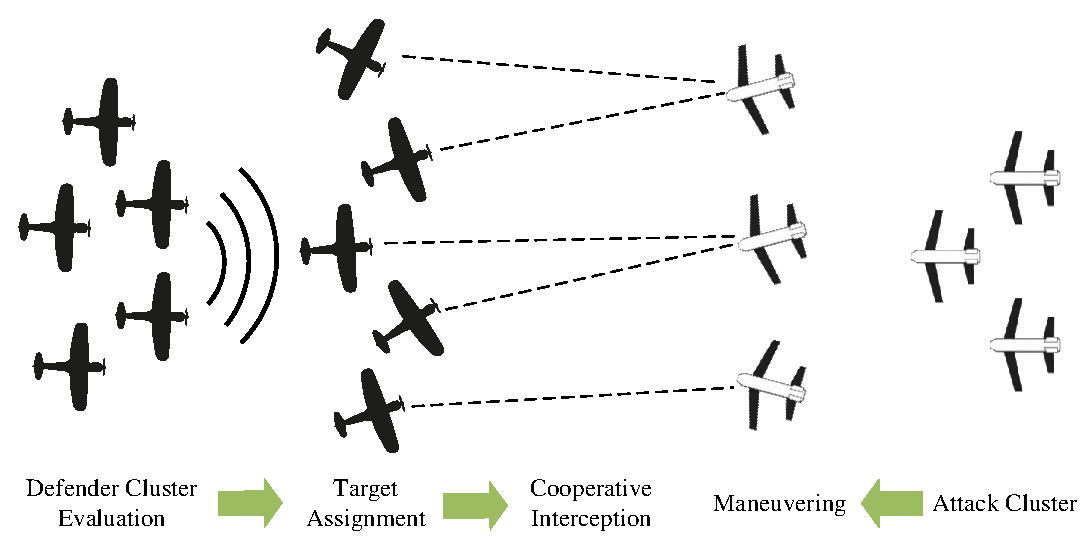
\includegraphics[width=2.8in]{fenpei.pdf}
\caption{Cluster target interception problem.}
\label{fenpei}
\end{figure}

The object of study in this paper is the fixed-wing UAV, and the interception problem is
reduced to a two-dimensional horizontal plane as shown in Fig.~\ref{jianmo} without loss of
generality.

\begin{figure}[!t]
\centering
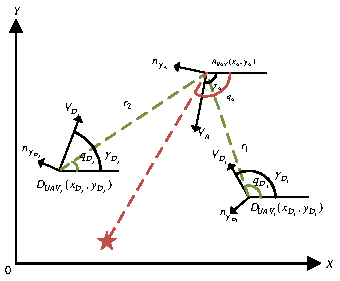
\includegraphics[width=2.6in]{pic02.pdf}
\caption{Schematic diagram of confrontation and interception.}
\label{jianmo}
\end{figure}

The kinematic model of a single UAV can be simplified as
\begin{equation}
\label{yundongxue}
\left\{\begin{matrix}\dot{x} =V\cos\gamma \\
\dot{y} =V\sin\gamma \end{matrix}\right.
\end{equation}
where \emph{x}, \emph{y} is the position coordinates of the UAV in two-dimensional space,
\emph{V} is the velocity magnitude of the UAV, and $\gamma$ is the navigation angle.

In an interception mission, the relative motion relationship between the attacking and
defending UAVs can be described as:
\begin{equation}
\label{gongfang}
\left\{\begin{matrix}\dot{r} =V_{A}\cos(\gamma_{A}-q)-V_{D}\cos(\gamma_{D}-q) \\
r\dot{q} =V_{A}\sin(\gamma_{A}-q)-V_{D}\sin(\gamma_{D}-q)\end{matrix}\right.
\end{equation}
where $r$ is the inter-UAV distance, $q$ is the line-of-sight angle, $V_{A}$ ($V_{D}$) is the
velocity of the attacking (defending) UAV, and $\gamma_{A}$ ($\gamma_{D}$) is the
corresponding heading angle.

In the interception phase, the relationship between UAV flight state and acceleration is:
\begin{equation}
\label{guozai}
\left\{\begin{matrix}\dot{V} =n_{x} g \\
\dot{\gamma} =n_{y}g/V \end{matrix}\right.
\end{equation}
where $n_{x}$ is the axial acceleration command, $n_{y}$ is the normal acceleration command,
and $g$ is the gravitational acceleration.
In the multi-agent setting of Section~\ref{sec:cooperative_algorithm}, these variables carry
an agent subscript $i$.

During cooperative interception, the remaining impact time is defined as:
\begin{equation}
\label{shijian}
t_{go}=\frac{r}{\left|\dot{r}\right|}
\end{equation}

The Zero-Effort Miss (ZEM) is defined as:
\begin{equation}
\label{ZEM}
ZEM = \frac{r^{2}\cdot\dot{q}}{\left|\dot{r}\right|}
\end{equation}

\subsection{Reinforcement Learning}

Reinforcement learning (RL) is built on the Markov Decision Process (MDP), comprising state
space $\mathcal{S}$, action space $\mathcal{A}$, reward function $R$, policy $\pi$, and state
transition function $P$.
At each step, the agent selects action $a$ from state $s$, receives reward $r$, and
transitions to $s'$.
The key value functions are:
\begin{equation}
\label{RLV}
V^{\pi}(s)=E_{\pi}\left[\sum_{t=0}^{\infty}\gamma_{\mathrm{RL}}^{t}r_{t}\mid s_{0}=s\right]
\end{equation}
\begin{equation}
\label{RLQ}
Q^{\pi}(s,a)=E_{\pi}\left[\sum_{t=0}^{\infty}\gamma_{\mathrm{RL}}^{t}r_{t}\mid s_{0}=s,a_{0}=a\right]
\end{equation}
where $\gamma_{\mathrm{RL}}\in[0,1]$ is the discount factor.






\section{Target Assignment via Distributed Consensus-Based IDBO Algorithm}
\label{sec:target_assignment}

This section formulates the cooperative target assignment as a weighted bipartite matching problem and solves it via an Improved Dung Beetle Optimization (IDBO) algorithm embedded in a distributed consensus framework.

\subsection{Problem Formulation}
\label{subsec:problem_formulation}

Let $\mathcal{U} = \{u_1, u_2, \dots, u_M\}$ and $\mathcal{T} = \{t_1, t_2, \dots, t_N\}$ denote the interceptor and target sets, respectively. Figure \ref{km} illustrates the bipartite assignment structure.

\begin{figure}[!t]
\centering
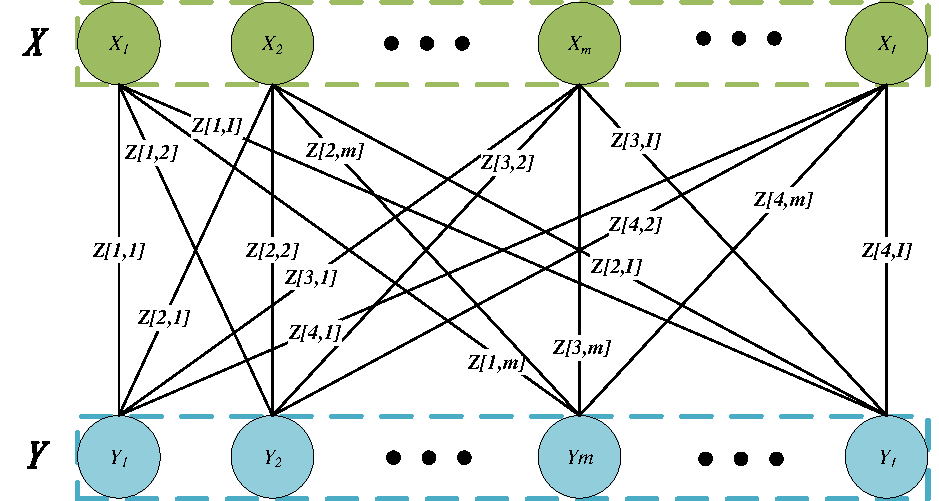
\includegraphics[width=2.5in]{KM1.pdf}
\caption{Schematic diagram of weighted dichotomy.}
\label{km}
\end{figure}

The binary decision variable $X_{ij}=1$ if UAV $u_i$ is assigned to target $t_j$ and 0 otherwise. The edge weight $P_{ij}$ quantifies the interception probability:

\begin{equation}
\label{eq:interception_probability}
P_{ij} = w_1 \cdot P_{\text{ZEM}}(i,j) + w_2 \cdot P_{\sigma}(i,j)
\end{equation}
where $w_1 + w_2 = 1$, $w_1, w_2 \geq 0$. The Zero-Effort Miss (ZEM) component is:

\begin{equation}
\label{eq:zem_prob}
P_{\text{ZEM}}(i,j) = \exp\left[-\frac{1}{2}\left(\frac{\text{ZEM}(i,j)}{\overline{\text{ZEM}}}\right)^2\right]
\end{equation}
where $\overline{\text{ZEM}} = \frac{1}{MN}\sum_{i=1}^{M}\sum_{j=1}^{N} \text{ZEM}(i,j)$.

The angular advantage component is:

\begin{equation}
\label{eq:angular_prob}
P_{\sigma}(i,j) = \exp\left[-\frac{1}{2}\left(\frac{S_{\sigma}(i,j)}{\overline{S_{\sigma}}}\right)^2\right]
\end{equation}
where $\overline{S_{\sigma}} = \frac{1}{MN}\sum_{i=1}^{M}\sum_{j=1}^{N} S_{\sigma}(i,j)$, with $S_{\sigma}(i,j) = |\gamma_{ij} - q_{ij}|$ denoting the heading error. The objective minimizes the expected number of surviving targets. Under many-to-one assignment, the joint survival probability of target $t_j$ is the product of individual failure probabilities:

\begin{equation}
\label{eq:optimization_formulation}
\begin{aligned}
\min_{\mathbf{X}} \quad & J = \sum_{j=1}^{N} \left[ \prod_{i=1}^{M} \left(1 - P_{ij}\right)^{X_{ij}} \right] \\
\text{s.t.} \quad & \sum_{j=1}^{N} X_{ij} = 1, \quad \forall i \in \{1,\dots,M\} \\
& \sum_{i=1}^{M} X_{ij} \geq 1, \quad \forall j \in \{1,\dots,N\} \\
& \sum_{i=1}^{M} X_{ij} \leq L_{\max}, \quad \forall j \in \{1,\dots,N\} \\
& X_{ij} \in \{0,1\}, \quad \forall i,j
\end{aligned}
\end{equation}
where $\prod_{i=1}^{M} (1 - P_{ij})^{X_{ij}}$ yields the survival probability of $t_j$, which decreases geometrically with the number of assigned interceptors.

\subsection{Distributed Consensus-Based IDBO Framework}
\label{subsec:idbo_algorithm}

The IDBO algorithm solves \eqref{eq:optimization_formulation} by alternating between local metaheuristic optimization and distributed consensus-based conflict resolution. Let $\mathbf{X}^{(k)} = [x_{ij}^{(k)}] \in \{0,1\}^{M \times N}$ denote the assignment matrix at iteration $k$, where $x_{ij}^{(k)}=1$ indicates UAV $u_i$ is assigned to target $t_j$. The integrated optimization is:

\begin{equation}
\label{eq:hierarchical}
\mathcal{A}_{\text{IDBO}}^{(k+1)} = \mathcal{G}_{\text{consensus}} \circ \mathcal{F}_{\text{optimizer}} \left( \mathbf{X}^{(k)}, \boldsymbol{\Theta}^{(k)} \right)
\end{equation}
where $\mathcal{F}_{\text{optimizer}}$ denotes the improved DBO operator and $\mathcal{G}_{\text{consensus}}$ the consensus-based conflict resolver. The parameter set $\boldsymbol{\Theta}^{(k)} = \{\mathbf{A}^{(k)}, \mathbf{P}^{(k)}, \mathbf{V}^{(k)}\}$ aggregates the adversarial advantage, interception probability, and velocity matrices at iteration $k$.

Each UAV $u_i$ maintains a preference vector $\mathbf{x}_i \in [0,1]^{N}$, where $x_{ij}$ encodes the normalized affinity for target $t_j$. The fitness function balances interception efficiency against resource saturation:

\begin{equation}
\label{eq:idbo_fitness}
\begin{split}
\mathcal{F}_i(\mathbf{x}_i) =& \sum_{j=1}^{N} \sigma(x_{ij}) \cdot P_{ij} + \lambda_1 \sum_{j=1}^{N} \sigma(x_{ij}) \cdot A_{ij} \\
&- \lambda_2 \sum_{j=1}^{N} \Psi_{ij}(\mathbf{x}_i, \hat{\mathbf{X}}_{\mathcal{N}_i})
\end{split}
\end{equation}
where the three terms correspond to interception probability, adversarial advantage ($\lambda_1$-weighted), and an over-saturation penalty ($\lambda_2$-weighted). The penalty $\Psi_{ij}$ is:

\begin{equation}
\label{eq:saturation_penalty}
\begin{split}
\Psi_{ij}(\mathbf{x}_i, \hat{\mathbf{X}}_{\mathcal{N}_i}) =& \sigma(x_{ij}) \cdot \max\Biggl(0, \Biggl(\sum_{k \in \mathcal{N}_i, k \neq i} \sigma(\hat{x}_{kj}) \\
&+ \sigma(x_{ij})\Biggr) - L_{\max}\Biggr)
\end{split}
\end{equation}
where $\mathcal{N}_i$ is the neighbor set of $u_i$, $\hat{x}_{kj}$ the estimated preference of neighbor $u_k$, and $L_{\max}$ the per-target interceptor capacity. The penalty activates only when the estimated assignment count exceeds $L_{\max}$, steering the swarm toward capacity-feasible solutions.

The adversarial advantage $A_{ij}$ fuses temporal, energetic, and geometric factors:

\begin{equation}
\label{eq:adversarial_advantage}
\begin{split}
A_{ij} =& \exp\left(-\frac{\Delta t_{ij}}{T_{\max}}\right) \cdot \left(1 - \frac{\|\mathbf{v}_i - \mathbf{v}_j\|_2}{v_{\max}}\right) \\
&\cdot \max\left(0, \cos(\theta_{ij})\right) - \sum_{k\neq i} \frac{P_{kj}}{P_{ij} + P_{kj}} \cdot \sigma(\hat{x}_{kj})
\end{split}
\end{equation}
where $\Delta t_{ij}$ is the estimated time-to-intercept; $\mathbf{p}_i=[x_i, y_i]^\top$ and $\mathbf{v}_i=[\dot{x}_i, \dot{y}_i]^\top$ denote the position and velocity vectors of interceptor $u_i$; $\mathbf{p}_j=[x_j, y_j]^\top$ and $\mathbf{v}_j=[\dot{x}_j, \dot{y}_j]^\top$ denote the position and velocity vectors of target $t_j$; $\theta_{ij}$ is the aspect angle associated with the engagement geometry between $u_i$ and $t_j$; and $v_{\max}$ is the maximum reference speed used for normalization. The three multiplicative factors encode temporal, energetic, and geometric advantage, respectively, while the subtracted term penalizes competition from other interceptors with high preferences for the same target.

The IDBO update mechanism enhances the standard DBO through four adversarial-information-driven operations:

\begin{align}
\text{Rolling:} \quad & \mathbf{x}_i^{(t+1)} = \mathbf{x}_i^{(t)} + \alpha \cdot \nabla_{\mathbf{x}_i} \mathcal{F}_i(\mathbf{x}_i^{(t)}) \circ \mathbf{A}_i \nonumber \\
& \quad + \beta \cdot \mathbf{r}_i \cdot \exp\left(-\frac{t}{T}\right) \label{eq:rolling_update} \\
\text{Dancing:} \quad & \mathbf{x}_i^{(t+1)} = \mathbf{x}_i^{(t)} \odot \exp\left(\gamma \cdot \tanh(\mathbf{A}_i - \bar{A}_i)\right) \nonumber \\
& \quad + \mathbf{n}_i, \quad \mathbf{n}_i \sim \mathcal{N}(0, \sigma_d^2 \mathbf{I}) \label{eq:dancing_update} \\
\text{Breeding:} \quad & \mathbf{x}_i^{(t+1)} = \mathbf{x}_i^{(t)} + \delta \cdot \left(\mathbf{x}_{\text{best}}^{(t)} - \mathbf{x}_i^{(t)}\right) \odot \mathbf{A}_i \nonumber \\
& \quad + \delta' \cdot \left(\mathbf{x}_{\text{second}}^{(t)} - \mathbf{x}_i^{(t)}\right) \label{eq:breeding_update} \\
\text{Stealing:} \quad & \mathbf{x}_i^{(t+1)} = \mathbf{x}_i^{(t)} \nonumber \\
& \quad + \eta \cdot \sum_{k \in \mathcal{K}_i} \frac{A_{ij}}{\sum_{l \in \mathcal{K}_i} A_{lj}} \cdot \left(\mathbf{x}_k^{(t)} - \mathbf{x}_i^{(t)}\right) \label{eq:stealing_update}
\end{align}
where $\mathbf{A}_i = [A_{i1}, A_{i2}, \dots, A_{iN}]^\top$, $\bar{A}_i$ is the mean of $\mathbf{A}_i$, $\mathbf{r}_i$ and $\mathbf{n}_i$ are random vectors, $\mathcal{K}_i$ represents UAVs competing for the same targets as $u_i$, and $\alpha, \beta, \gamma, \delta, \delta', \eta$ are adaptive coefficients that decay linearly with iteration $t$. Continuous preferences are binarized via advantage-adaptive thresholding:

\begin{equation}
\label{eq:thresholding}
X_{ij} = 
\begin{cases}
1, & \text{if } \sigma(x_{ij}) > \tau \cdot \left(1 + \frac{A_{ij}}{\max_k A_{ik}}\right) \\
0, & \text{otherwise}
\end{cases}
\end{equation}
where $\tau \in (0,1)$ is a base threshold. Each UAV maintains a bundle $\mathcal{B}_i$, bid vector $\mathbf{c}_i = [c_{i1}, \dots, c_{iN}]$, winner list $\mathbf{z}_i = [z_{i1}, \dots, z_{iN}]$, and timestamp vector $\mathbf{y}_i = [y_{i1}, \dots, y_{iN}]$. The bid for target $t_j$ governs the distributed auction:

\begin{equation}
\label{eq:bid_formulation}
c_{ij} = \mathcal{F}_i(\mathbf{x}_i) \cdot \sigma(x_{ij}) \cdot \exp\left(\frac{A_{ij} - \bar{A}_i}{\sigma_A}\right)
\end{equation}
where $\bar{A}_i$ and $\sigma_A$ are the mean and standard deviation of $u_i$'s adversarial advantages. The fitness--preference product captures local assignment quality, while the exponential term amplifies bids for targets where $u_i$ holds above-average advantage. To support cooperative saturation attacks, the consensus mechanism employs top-$K$ bidding. Each UAV maintains a winner list $\mathcal{Z}_{j} = \{(u_k, c_{kj})\}$ for $t_j$, containing up to $L_{\max}$ highest bids:

\begin{equation}
\label{eq:cbba_update}
\mathcal{Z}_{j}^{(k+1)} = \text{Top}_{L_{\max}} \left( \mathcal{Z}_{j}^{(k)} \cup \bigcup_{l \in \mathcal{N}_i} \mathcal{Z}_{j,l}^{(k)} \cup \{(u_i, c_{ij}^{(k+1)})\} \right)
\end{equation}
where $\text{Top}_{L_{\max}}(\cdot)$ retains the $L_{\max}$ highest-bid entries. UAV $u_i$ secures a slot for $t_j$ if $|\mathcal{Z}_{j}| < L_{\max}$ or its bid exceeds $\min_{(u_k, c_{kj}) \in \mathcal{Z}_{j}} c_{kj}$, thereby displacing the weakest contributor and prioritizing the most capable interceptors.

As depicted in the procedural flowchart (Fig.~\ref{fig:idbo_flowchart}), the algorithm iterates over three interleaved phases—local optimization (Eqs.~\ref{eq:rolling_update}--\ref{eq:stealing_update}), consensus resolution (Eqs.~\ref{eq:thresholding}--\ref{eq:cbba_update}), and advantage update—until convergence:

\begin{align}
\text{Phase 1: } & \mathbf{x}_i^{(k+1)} = \mathcal{F}_{\text{optimizer}}\left(\mathbf{x}_i^{(k)}, \mathcal{F}_i, \mathbf{A}_i^{(k)}, \mathbf{P}^{(k)}\right) \label{eq:phase1} \\
\text{Phase 2: } & \{\mathbf{z}_i^{(k+1)}, \mathcal{B}_i^{(k+1)}\} = \nonumber \\ 
& \mathcal{G}_{\text{consensus}}\left(\{\sigma(\mathbf{x}_i^{(k+1)})\}, \{\mathbf{c}_i^{(k+1)}\}, \{\mathbf{y}_i^{(k)}\}\right) \label{eq:phase2} \\
\text{Phase 3: } & \mathbf{A}_i^{(k+1)} = \mathcal{H}\left(\mathbf{z}_i^{(k+1)}, \mathcal{B}_i^{(k+1)}, \mathbf{V}_i^{(k+1)}, \mathbf{V}_T^{(k+1)}\right) \label{eq:phase3}
\end{align}

\begin{figure}[!t]
\centering
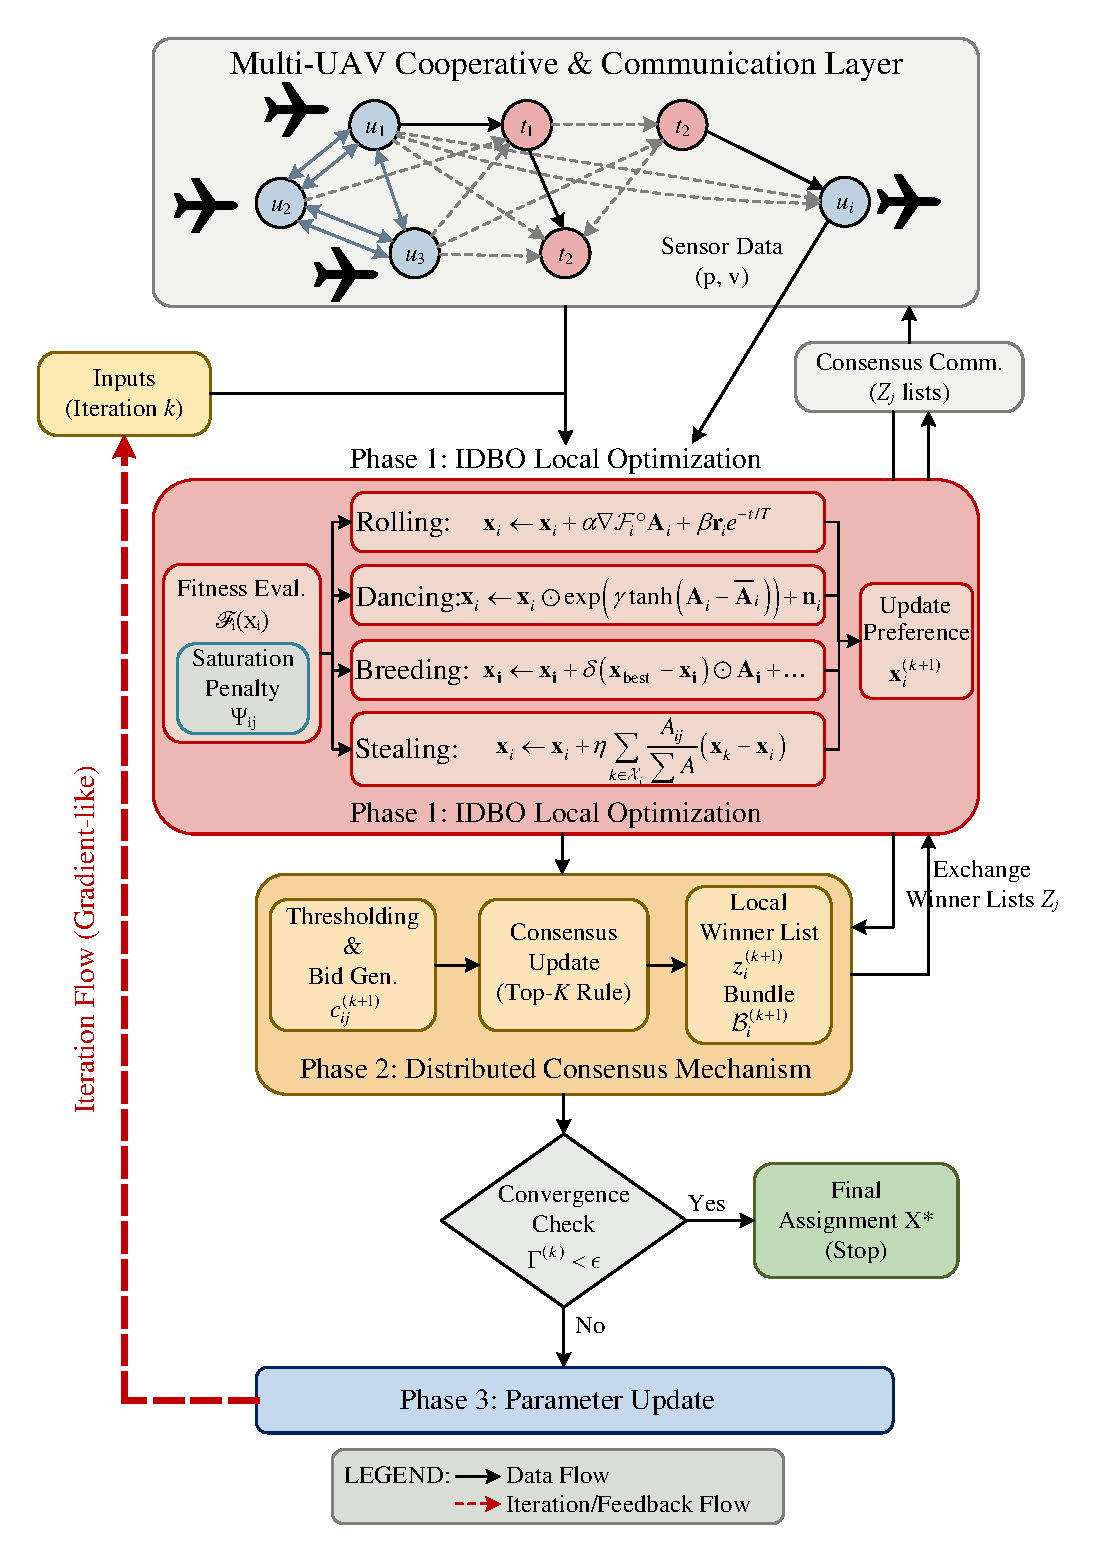
\includegraphics[width=3.2in]{assignment.pdf}
\caption{Flowchart of the distributed consensus-based IDBO algorithm, illustrating the algorithmic iteration flow across local metaheuristic optimization, auction-based consensus, and adversarial information updates.}
\label{fig:idbo_flowchart}
\end{figure}

Here, $\mathcal{H}$ updates adversarial advantages given the consensus assignment and velocity vectors $\mathbf{V}_i$, $\mathbf{V}_T$. Following the iteration flow in Fig.~\ref{fig:idbo_flowchart}, convergence is declared when the swarm-wide assignment disagreement falls below $\epsilon$:

\begin{equation}
\label{eq:convergence}
\Gamma^{(k)} = \frac{1}{M} \sum_{i=1}^{M} \left\| \mathbf{z}_i^{(k)} - \frac{1}{|\mathcal{N}_i|} \sum_{j \in \mathcal{N}_i} \mathbf{z}_j^{(k)} \right\|_0 < \epsilon
\end{equation}
where $\|\cdot\|_0$ counts disagreeing entries and $\epsilon$ is a convergence threshold. The algorithm guarantees monotonic fitness improvement: $\Phi^{(k+1)} \geq \Phi^{(k)}$ a.s., where $\Phi^{(k)} = \sum_{i=1}^{M} \mathcal{F}_i(\mathbf{x}_i^{(k)})$. Under a connected communication graph with finite message delays, consensus is reached in at most $N \cdot D$ iterations ($D$: graph diameter). The converged assignment $\mathbf{X}^*$ constitutes an $\epsilon$-approximate Nash equilibrium: $\mathcal{F}_i(\mathbf{x}_i^*) \geq \mathcal{F}_i(\mathbf{x}_i') - \epsilon$, $\forall \mathbf{x}_i' \in \mathcal{X}_i$, $\forall i$.

The per-UAV per-iteration complexity decomposes as:

\begin{equation}
\label{eq:complexity}
C_{\text{total}} = O(T \cdot P \cdot N^2) + O(N \cdot |\mathcal{N}_i|) + O(N)
\end{equation}
where $T$ is the IDBO iteration count, $P = O(N)$ the population size, and $|\mathcal{N}_i|$ the neighborhood size. The three terms account for optimization, consensus communication, and advantage update, respectively. Communication cost is $O(N \cdot |\mathcal{N}_i|)$ and memory is $O(P \cdot N + N)$ per UAV.













%% ===========================================================
\section{ART-MAPPO: Attention-Residual and Trust-Aware MAPPO for Cooperative Swarm Interception}
\label{sec:cooperative_algorithm}

Building on the distributed consensus-based IDBO target assignment, we propose the Attention-Residual and Trust-aware MAPPO (ART-MAPPO) algorithm for the cooperative guidance of defending UAV swarms under the Centralized Training with Decentralized Execution (CTDE) paradigm. ART-MAPPO augments the standard MAPPO framework with three synergistic modules: a kinematics-aware attention-residual network for extracting cross-coupled engagement features, a trust-modulated exploration mechanism for discovering cooperative tactics within the safe flight envelope, and a dual-clip PPO with adaptive KL penalty for constraining guidance command variations against actuator saturation.

\subsection{Enhanced Situational Awareness via Attention-Residual Network}
\label{subsec:attention_residual}

The highly dynamic nature of swarm interception requires interceptors to process complex, coupled kinematic states. Let $\mathbf{o}_i^{(t)} \in \mathbb{R}^{n_o}$ denote the observation vector for interceptor $i$ at time step $t$, as defined in Section~\ref{subsec:state_reward}. A base feature encoder $f_{\mathrm{enc}}$, comprising a two-layer MLP with hidden dimension $d_{\mathrm{enc}}$ and Layer Normalization, projects the raw observation into a high-dimensional latent space:
\begin{equation}
\label{eq:encoder}
\begin{split}
\mathbf{h}^{(0)} =& \operatorname{LN}\Bigl(\operatorname{ReLU}\bigl(\mathbf{o}_i^{(t)}\mathbf{W}_{\mathrm{enc}}^{(1)} + \mathbf{b}_{\mathrm{enc}}^{(1)}\bigr) \\
&\cdot \mathbf{W}_{\mathrm{enc}}^{(2)} + \mathbf{b}_{\mathrm{enc}}^{(2)}\Bigr) \in \mathbb{R}^{d}
\end{split}
\end{equation}
where $\mathbf{W}_{\mathrm{enc}}^{(1)} \in \mathbb{R}^{n_o \times d_{\mathrm{enc}}}$ and $\mathbf{W}_{\mathrm{enc}}^{(2)} \in \mathbb{R}^{d_{\mathrm{enc}} \times d}$ are learnable projection matrices.

\emph{1) Kinematics-Aware Multi-Head Attention:} To capture the nonlinear spatio-temporal coupling among engagement variables (e.g., the interdependence between LOS rate $\dot{q}$ and time-to-go synchronization), we reshape $\mathbf{h}^{(0)}$ into a sequence of $n_o$ feature tokens $\mathbf{H}^{(0)} \in \mathbb{R}^{n_o \times (d/n_o)}$ and apply multi-head self-attention. For each head $j \in \{1, \dots, H\}$, the query, key, and value projections are:
\begin{equation}
\label{eq:qkv}
\mathbf{Q}_j = \mathbf{H}^{(0)}\mathbf{W}_j^{Q}, \quad \mathbf{K}_j = \mathbf{H}^{(0)}\mathbf{W}_j^{K}, \quad \mathbf{V}_j = \mathbf{H}^{(0)}\mathbf{W}_j^{V}
\end{equation}
where $\mathbf{W}_j^{Q}, \mathbf{W}_j^{K} \in \mathbb{R}^{(d/n_o) \times d_k}$ and $\mathbf{W}_j^{V} \in \mathbb{R}^{(d/n_o) \times d_v}$, with $d_k = d_v = d/H$. The scaled dot-product attention for head $j$, incorporating an observability mask $\mathbf{M} \in \mathbb{R}^{n_o \times n_o}$, is:
\begin{align}
\mathbf{A}_j &= \mathrm{softmax}\!\left(\frac{\mathbf{Q}_j\mathbf{K}_j^\top}{\sqrt{d_k}} + \mathbf{M}\right) \in \mathbb{R}^{n_o \times n_o} \label{eq:attention} \\
\mathrm{head}_j &= \mathbf{A}_j\mathbf{V}_j \in \mathbb{R}^{n_o \times d_v} \nonumber
\end{align}
where $M_{u,v} = -\infty$ isolates unobservable kinematic channels (e.g., LOS rate during sensor blanking) and $M_{u,v} = 0$ permits information flow. The multi-head outputs are concatenated, projected, and added back via a residual shortcut:
\begin{equation}
\label{eq:mha_out}
\begin{split}
\mathbf{h}_{\mathrm{attn}} =& \mathbf{h}^{(0)} + \mathrm{Dropout}_{p}\Bigl(\operatorname{Flatten}\bigl( \\
&\left[\mathrm{head}_1 \| \cdots \| \mathrm{head}_H\right]\bigr) \mathbf{W}^{O}\Bigr)
\end{split}
\end{equation}
where $\mathbf{W}^{O} \in \mathbb{R}^{d \times d}$ is the output projection and $\operatorname{Flatten}(\cdot)$ reshapes the token sequence back to $\mathbb{R}^d$. The residual connection ensures that primitive flight-state components propagate losslessly to downstream layers.

\emph{2) Residual Block with Layer Normalization:} To deepen the nonlinear representational capacity without gradient vanishing---a critical issue when extreme overload commands produce large-magnitude gradients---a stack of $L$ residual blocks follows the attention module. For the $\ell$-th block ($\ell \in \{1, \dots, L\}$) with input $\mathbf{h}^{(\ell)}$ (where $\mathbf{h}^{(1)} = \mathbf{h}_{\mathrm{attn}}$), the forward pass is:
\begin{align}
\mathbf{z}_1^{(\ell)} &= \operatorname{ReLU} \left( \operatorname{LN}_1^{(\ell)} \left( \mathbf{h}^{(\ell)}\mathbf{W}_1^{(\ell)} + \mathbf{b}_1^{(\ell)} \right) \right) \label{eq:res_block_inner1} \\
\mathbf{z}_2^{(\ell)} &= \operatorname{LN}_2^{(\ell)} \left( \mathbf{z}_1^{(\ell)}\mathbf{W}_2^{(\ell)} + \mathbf{b}_2^{(\ell)} \right) \label{eq:res_block_inner2} \\
\mathbf{h}^{(\ell+1)} &= \operatorname{ReLU} \left( \mathbf{z}_2^{(\ell)} + \mathbf{h}^{(\ell)} \right) \label{eq:res_block_out}
\end{align}
where $\mathbf{W}_1^{(\ell)}, \mathbf{W}_2^{(\ell)} \in \mathbb{R}^{d \times d}$ are orthogonally initialized. The identity shortcut yields the Jacobian:
\begin{equation}
\label{eq:jacobian}
\begin{split}
\frac{\partial \mathbf{h}^{(\ell+1)}}{\partial \mathbf{h}^{(\ell)}} =& \operatorname{diag}\!\left(\mathbb{I}\!\left[\mathbf{z}_2^{(\ell)} + \mathbf{h}^{(\ell)} > \mathbf{0}\right]\right) \\
&\cdot \left(\mathbf{I} + \frac{\partial \mathbf{z}_2^{(\ell)}}{\partial \mathbf{h}^{(\ell)}}\right)
\end{split}
\end{equation}
Since the ReLU gate preserves the identity component on active units, gradient norms satisfy $\left\|\frac{\partial \mathbf{h}^{(\ell+1)}}{\partial \mathbf{h}^{(\ell)}}\right\| \geq \left\|\operatorname{diag}(\mathbb{I}[\cdot])\right\| > 0$, preventing vanishing gradients across $L$ blocks.

\emph{3) End-to-End Guidance Command Generation:} The refined feature $\mathbf{h}^{(L+1)}$ is fed into a GRU cell to integrate temporal engagement history:
\begin{equation}
\label{eq:gru}
\mathbf{c}_t = \operatorname{GRU}\!\left(\mathbf{h}^{(L+1)},\, \mathbf{c}_{t-1};\, \mathbf{W}_{\mathrm{GRU}}\right), \quad \mathbf{c}_t \in \mathbb{R}^{d_{\mathrm{rnn}}}
\end{equation}
where $\mathbf{W}_{\mathrm{GRU}}$ denotes the GRU parameters and $\mathbf{c}_{t-1}$ is the hidden state from the previous guidance step. The actor network then parameterizes a diagonal Gaussian over the continuous overload action space:
\begin{equation}
\label{eq:actor_dist}
\begin{split}
\pi_{\theta_i}\!\left(a_i \mid \mathbf{o}_i^{(t)}\right) &= \mathcal{N}\!\left(\boldsymbol{\mu}_{\theta_i}(\mathbf{c}_t),\; \operatorname{diag}\!\left(\boldsymbol{\sigma}_{\theta_i}^2(\mathbf{c}_t)\right)\right) \\
a_i &= [n_{x_i},\, n_{y_i}]^\top \in \mathcal{A}
\end{split}
\end{equation}
where $\boldsymbol{\mu}_{\theta_i}, \boldsymbol{\sigma}_{\theta_i}^2: \mathbb{R}^{d_{\mathrm{rnn}}} \to \mathbb{R}^2$ are linear output heads. The action is clipped to the feasible envelope $\mathcal{A}$ after sampling. Concurrently, the centralized critic shares the same attention-residual backbone but receives the concatenated global state:
\begin{equation}
\label{eq:critic_input}
s_t = \left[\mathbf{o}_1^{(t)} \| \mathbf{o}_2^{(t)} \| \cdots \| \mathbf{o}_N^{(t)}\right] \in \mathbb{R}^{N \cdot n_o}
\end{equation}
to produce the state-value estimate $V_\phi(s_t) \in \mathbb{R}$, enabling centralized advantage computation during training while each actor executes independently from local observations $\mathbf{o}_i^{(t)}$ at deployment.

\subsection{Trust-Modulated Tactical Exploration}
\label{subsec:trust_exploration}

Based on the high-fidelity features extracted by the attention-residual backbone, we introduce a trust-based mechanism to dynamically modulate the exploration policy. This mechanism mathematically balances the exploitation of known guidance laws against the discovery of complex cooperative tactics (e.g., flanking or simultaneous impact).

\emph{1) Trust Evolution:} Let $R_i^{(k)} = \sum_{t=0}^{T} \gamma_{\mathrm{RL}}^t r_i^{(t)}$ be the discounted cumulative return of interceptor $i$ in episode $k$, where $\gamma_{\mathrm{RL}} \in (0,1)$ is the RL discount factor (distinct from the heading angle $\gamma_{D_i}$) and $T$ is the episode horizon. The swarm-level running statistics are maintained as exponential moving averages:
\begin{align}
\mu_R &\leftarrow (1-\rho)\,\mu_R + \rho\,\frac{1}{N}\sum_{i=1}^{N} R_i^{(k)} \label{eq:running_stats_mu} \\
\sigma_R^2 &\leftarrow (1-\rho)\,\sigma_R^2 + \rho\,\frac{1}{N}\sum_{i=1}^{N}\!\left(R_i^{(k)} - \mu_R\right)^2 \label{eq:running_stats_sigma}
\end{align}
where $\rho \in (0,1)$ is the statistics update rate. The normalized relative performance of interceptor $i$ is then:
\begin{equation}
\label{eq:trust_normalized}
\tilde{R}_i^{(k)} = \frac{R_i^{(k)} - \mu_R}{\sqrt{\sigma_R^2 + \epsilon_0}}
\end{equation}
where $\epsilon_0 > 0$ is a numerical stabilizing constant. The trust level $\mathcal{T}_i^{(k)} \in (0,1)$ evolves via first-order exponential smoothing with a sigmoid activation:
\begin{equation}
\label{eq:trust_evolution}
\mathcal{T}_i^{(k+1)} = (1-\alpha_T)\,\mathcal{T}_i^{(k)} + \alpha_T\,\sigma\!\left(\tau_T \tilde{R}_i^{(k)}\right)
\end{equation}
where $\sigma(x) = 1/(1+e^{-x})$, $\alpha_T \in (0,1)$ is the trust update rate and $\tau_T > 0$ is the temperature parameter controlling the sensitivity of trust to performance deviations. When $R_i^{(k)} > \mu_R$, the sigmoid output exceeds 0.5, driving $\mathcal{T}_i$ upward and reducing exploration; conversely, below-average performance lowers $\mathcal{T}_i$ and amplifies exploration.

\emph{2) Blended Exploration Policy:} The final action for interceptor $i$ is drawn from a two-component mixture: with probability $1-\beta(\mathcal{T}_i)$ from the learned policy, and with probability $\beta(\mathcal{T}_i)$ from a structured heuristic distribution, i.e.,
\begin{equation}
\label{eq:exploration_policy}
a_i \sim \begin{cases} \pi_{\theta_i}(\cdot \mid \mathbf{o}_i^{(t)}) & \text{with prob. } 1 - \beta(\mathcal{T}_i) \\ \pi_{\mathrm{guided}}^{i}(\cdot \mid \mathbf{o}_i^{(t)}) & \text{with prob. } \beta(\mathcal{T}_i) \end{cases}
\end{equation}
where the modulation factor $\beta(\mathcal{T}_i) = 1 - \mathcal{T}_i \in (0,1)$ is monotonically decreasing in trust. The heuristic distribution $\pi_{\mathrm{guided}}^{i}$ is a discrete mixture over three tactically informative actions within the feasible command space $\mathcal{A} = [n_{x}^{\min}, n_{x}^{\max}] \times [n_{y}^{\min}, n_{y}^{\max}]$:
\begin{equation}
\label{eq:guided}
\begin{split}
\pi_{\mathrm{guided}}^{i}(a_i \mid \mathbf{o}_i^{(t)}) =& \omega_1\,\delta(a_i - a_{\mathrm{opt}}) + \omega_2\,\delta(a_i - a_{\mathrm{probe}}) \\
&+ \omega_3\,\mathcal{U}(\mathcal{A}), \quad \sum_{k=1}^3\omega_k=1
\end{split}
\end{equation}
Here, $a_{\mathrm{opt}} = \arg\max_{a \in \mathcal{A}} Q_\phi(\mathbf{o}_i^{(t)}, a)$ mimics the classical proportional navigation command for exploitation, $a_{\mathrm{probe}} = \arg\min_{a \in \mathcal{A}} Q_\phi(\mathbf{o}_i^{(t)}, a)$ deliberately executes extreme boundary maneuvers to probe the aerodynamic envelope, and $\mathcal{U}(\mathcal{A})$ maintains stochastic coverage of the remaining action space. The expected action under the full mixture policy is:
\begin{equation}
\label{eq:expected_action}
\begin{split}
\mathbb{E}[a_i] =& \bigl(1-\beta(\mathcal{T}_i)\bigr)\,\boldsymbol{\mu}_{\theta_i}(\mathbf{c}_t) \\
&+ \beta(\mathcal{T}_i)\,\bigl(\omega_1\,a_{\mathrm{opt}} + \omega_2\,a_{\mathrm{probe}} + \omega_3\,\bar{a}_{\mathcal{A}}\bigr)
\end{split}
\end{equation}
where $\bar{a}_{\mathcal{A}} = \frac{1}{2}[n_x^{\min}+n_x^{\max},\; n_y^{\min}+n_y^{\max}]^\top$ is the centroid of $\mathcal{A}$.

\subsection{Robust Optimization via Dual-Clip and Adaptive KL}
\label{subsec:dual_clip_kl}

Aggressive exploration inherently induces substantial variations in the importance-sampling ratio $r_t(\theta) = \pi_\theta(a_t \mid o_t) / \pi_{\theta_{\mathrm{old}}}(a_t \mid o_t)$, leading to oscillatory terminal overload commands $n_{y_i}$ that can severely compromise flight stability. We stabilize policy gradient optimization using a dual-clip surrogate objective combined with an adaptive KL divergence penalty.

\emph{1) Generalized Advantage Estimation:} The advantage $\hat{A}_t$ is computed via GAE with discount $\gamma_{\mathrm{RL}}$ and trace-decay $\lambda_{\mathrm{GAE}} \in [0,1]$:
\begin{align}
\hat{A}_t &= \sum_{l=0}^{T-t-1} (\gamma_{\mathrm{RL}}\lambda_{\mathrm{GAE}})^l \delta_{t+l} \label{eq:gae_A} \\
\delta_t &= r_i^{(t)} + \gamma_{\mathrm{RL}} V_\phi(s_{t+1}) - V_\phi(s_t) \label{eq:gae_delta}
\end{align}
where $\delta_t$ is the TD residual. The corresponding value target is $\hat{V}_t^{\mathrm{targ}} = \hat{A}_t + V_\phi(s_t)$.

\emph{2) Dual-Clip PPO Objective:} The standard clipped surrogate is:
\begin{equation}
\label{eq:standard_clip}
\begin{split}
L^{\mathrm{CLIP}}(\theta) = \min \Bigl( &r_t(\theta)\hat{A}_t, \\
&\operatorname{clip}\!\left(r_t(\theta), 1-\epsilon, 1+\epsilon\right)\hat{A}_t \Bigr)
\end{split}
\end{equation}
where $\epsilon \in (0,1)$ is the clipping threshold. When $\hat{A}_t < 0$, the standard clip permits $r_t(\theta) \to \infty$, causing catastrophic over-correction of overload commands. The Dual-Clip objective addresses this by introducing a floor $c > 1+\epsilon$ applied only when $\hat{A}_t < 0$:
\begin{equation}
\label{eq:dual_clip_final}
J^{\mathrm{DC}}(\theta) = \mathbb{E}_{t} \left[
\begin{cases}
\max\!\left( L^{\mathrm{CLIP}}(\theta),\; c\,\hat{A}_t \right) & \hat{A}_t < 0 \\[4pt]
L^{\mathrm{CLIP}}(\theta) & \hat{A}_t \geq 0
\end{cases}
\right]
\end{equation}
When $\hat{A}_t < 0$, the $\max$ with $c\,\hat{A}_t$ bounds $r_t(\theta) \leq c$, preventing the policy from over-penalizing actions that only marginally degrade performance. When $\hat{A}_t \geq 0$, the standard pessimistic clip suffices. The effective constraint on $r_t(\theta)$ under the dual-clip is therefore:
\begin{equation}
\label{eq:rt_bound}
r_t(\theta) \in \begin{cases} \left[\frac{1}{c},\; c\right] & \hat{A}_t < 0 \\[4pt] \left[1-\epsilon,\; 1+\epsilon\right] & \hat{A}_t \geq 0 \end{cases}
\end{equation}

\emph{3) Adaptive KL Regularization:} To continuously constrain policy deviation between updates, the KL divergence is approximated as:
\begin{equation}
\label{eq:kl_approx}
\begin{split}
\hat{D}_{\mathrm{KL}}\!\left(\pi_{\theta_{\mathrm{old}}} \| \pi_\theta\right) &= \mathbb{E}_t\!\left[\log\frac{\pi_{\theta_{\mathrm{old}}}(a_t \mid o_t)}{\pi_\theta(a_t \mid o_t)}\right] \\
&= \mathbb{E}_t\!\left[\log\pi_{\theta_{\mathrm{old}}}(a_t \mid o_t) - \log\pi_\theta(a_t \mid o_t)\right]
\end{split}
\end{equation}
The penalty coefficient $\beta_{\mathrm{KL}}$ is updated after each training epoch $k$ via:
\begin{equation}
\label{eq:kl_adapt}
\beta_{\mathrm{KL}}^{(k+1)} =
\begin{cases}
\min\!\left(1.5\,\beta_{\mathrm{KL}}^{(k)},\; \beta_{\max}\right), & \hat{D}_{\mathrm{KL}} > 2\,\delta_{\mathrm{targ}} \\[6pt]
\max\!\left(0.9\,\beta_{\mathrm{KL}}^{(k)},\; \beta_{\min}\right), & \hat{D}_{\mathrm{KL}} < 0.5\,\delta_{\mathrm{targ}} \\[6pt]
\beta_{\mathrm{KL}}^{(k)}, & \text{otherwise}
\end{cases}
\end{equation}
where $\delta_{\mathrm{targ}}$ is the target KL constraint, and $\beta_{\max}=10$, $\beta_{\min}=10^{-4}$ prevent the regularization from dominating or vanishing. When $\hat{D}_{\mathrm{KL}} > 2\delta_{\mathrm{targ}}$, the overload commands have shifted too aggressively between updates, risking structural load-factor exceedance; the $1.5\times$ increase dampens subsequent updates. When $\hat{D}_{\mathrm{KL}} < 0.5\delta_{\mathrm{targ}}$, the $0.9\times$ decay permits finer trajectory refinement.

\emph{4) Overall Loss Formulation:} The critic value loss over a mini-batch of size $B$ is:
\begin{equation}
\label{eq:value_loss}
L_V(\phi) = \frac{1}{B}\sum_{t=1}^{B} \left(V_\phi(s_t) - \hat{V}_t^{\mathrm{targ}}\right)^2
\end{equation}
Combining the dual-clip surrogate, adaptive KL penalty, value loss, and policy entropy bonus $S[\pi_\theta] = -\mathbb{E}_t[\log\pi_\theta(a_t \mid o_t)]$, the unified loss minimized by AdamW with cosine annealing is:
\begin{equation}
\label{eq:total_loss}
\mathcal{L}(\theta,\phi) = - J^{\mathrm{DC}}(\theta) + \beta_{\mathrm{KL}}\,\hat{D}_{\mathrm{KL}} + c_v\,L_V(\phi) - c_e\,S[\pi_\theta]
\end{equation}
where $c_v > 0$ and $c_e > 0$ are the value and entropy weighting coefficients. The learning rate follows a cosine annealing schedule $\eta(k) = \eta_{\min} + \frac{1}{2}(\eta_0 - \eta_{\min})(1 + \cos(\pi k / K))$, facilitating coarse trajectory optimization early in training and fine-grained terminal-guidance refinement in later epochs.

The complete ART-MAPPO workflow, integrating all three modules described above, is illustrated in Fig.~\ref{fig:algorithm_flow}.

\begin{figure*}[!t]
\centering
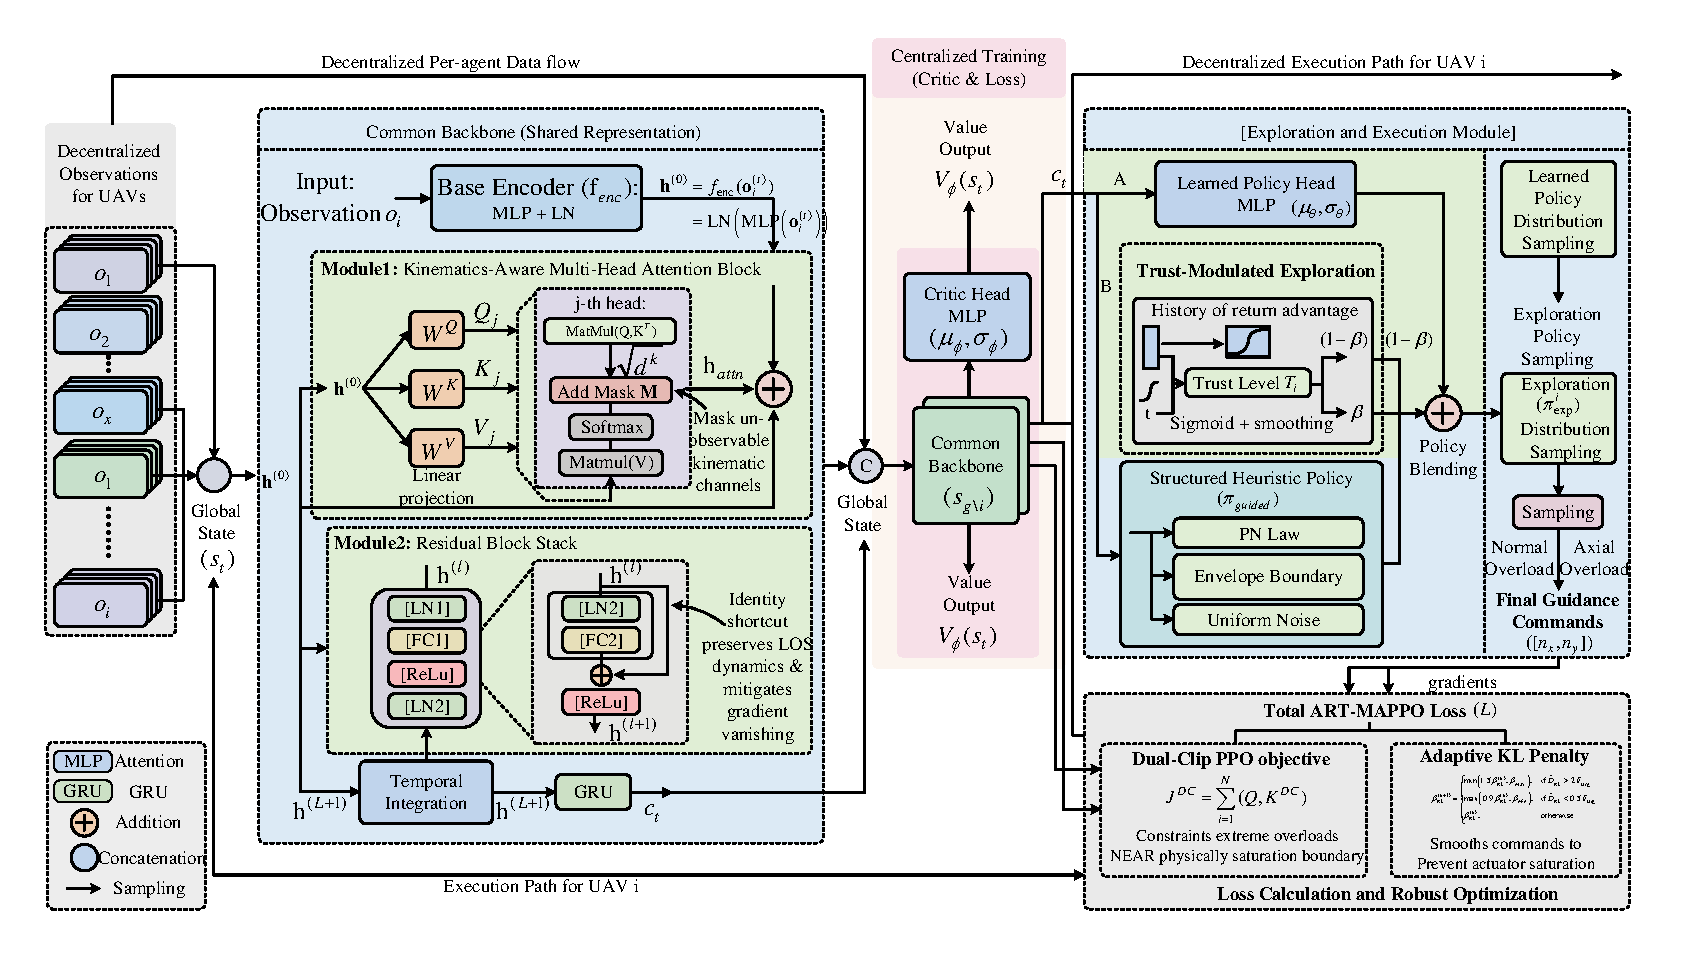
\includegraphics[width=7.3in]{rlsuanfa.pdf}
\caption{Overall workflow of the ART-MAPPO algorithm for cooperative swarm interception, showing the interaction among the attention-residual network, trust-modulated exploration, and dual-clip adaptive KL optimization.}
\label{fig:algorithm_flow}
\end{figure*}

\subsection{State Representation and Reward Design}
\label{subsec:state_reward}

\emph{1) Observation Space:} The observation vector for interceptor $i$ at time step $t$ is designed to capture the essential kinematic quantities for guidance and coordination:
\begin{equation}
\label{eq:observation_space}
\mathbf{o}_i^{(t)} = \left[o_i^{(t),1},\; o_i^{(t),2},\; o_i^{(t),3},\; o_i^{(t),4}\right]^\top \in \mathbb{R}^{n_o},\quad n_o = 4
\end{equation}
The four components are defined as:
% \begin{align}
% o_i^{(t),1} &= \begin{cases} \dfrac{V_i \dot{q}_t}{g}, & |\dot{q}_t - \dot{q}_{t-1}| \leq \Delta\dot{q}_{\max} \\[6pt] \dfrac{V_i \dot{q}_{t-1}}{g}, & |\dot{q}_t - \dot{q}_{t-1}| > \Delta\dot{q}_{\max} \end{cases} \label{eq:o1} \\[6pt]
% o_i^{(t),2} &= \gamma_{D_i} - q_i \label{eq:o2} \\[4pt]
% o_i^{(t),3} &= \left(n_{x_i}^2 + n_{y_i}^2\right) \cdot \Delta t \label{eq:o3} \\[4pt]
% o_i^{(t),4} &= \frac{r_i}{\min_{j \in \mathcal{G}_i} t_{go_j}} - V_i \label{eq:o4}
% \end{align}
\begin{align}
o_i^{(t),1} &=
\begin{cases}
\dfrac{V_i \dot{q}_i^{(t)}}{g}, &
\left|\dot{q}_i^{(t)} - \dot{q}_i^{(t-1)}\right| \leq \Delta \dot{q}_{\max}
\\[6pt]
\dfrac{V_i \dot{q}_i^{(t-1)}}{g}, &
\left|\dot{q}_i^{(t)} - \dot{q}_i^{(t-1)}\right| > \Delta \dot{q}_{\max}
\end{cases}
\label{eq:o1}
\\[6pt]
o_i^{(t),2} &= \gamma_{D_i} - q_i
\label{eq:o2}
\\[4pt]
o_i^{(t),3} &= \left(n_{x_i}^2 + n_{y_i}^2\right)\cdot \Delta t
\label{eq:o3}
\\[4pt]
o_i^{(t),4} &= \frac{r_i}{\min_{j \in \mathcal{G}_i} t_{go_j}} - V_i
\label{eq:o4}
\end{align}
where $\Delta\dot{q}_{\max} = 0.03$~rad/s is the LOS-rate noise threshold, $\mathcal{G}_i$ denotes the set of interceptors assigned to the same target as interceptor $i$, and $\Delta t$ is the simulation timestep. 
Component $o_i^{(t),1}$ is a smoothed required normal acceleration proportional to $V_i \dot{q}_i^{(t)} / g$, where the previous LOS-rate estimate is retained when the instantaneous measurement jump exceeds $\Delta \dot{q}_{\max}$.
Component $o_i^{(t),2}$ is the lead-angle deviation driving heading correction, where $q_i$ (and its derivative $\dot{q}_i$) denotes the specific line-of-sight (LOS) angle between interceptor $i$ and its dynamically assigned target. 
Component $o_i^{(t),3}$ encodes the instantaneous control energy expenditure. 
Component $o_i^{(t),4}$ is the velocity error relative to the desired approach speed $r_i / \min_j t_{go_j}$, which drives time-coordinated impact.




\emph{2) Reward Function:} The reward function incorporates five components to guide the learning process:
\begin{equation}
\label{eq:reward_function}
\begin{split}
r_i^{(t)} =& \; w_1 r_i^{\text{dist}} + w_2 r_i^{\text{angle}} + w_3 r_i^{\text{hit}} \\
&+ w_4 r_i^{\text{coord}} + w_5 r_i^{\text{energy}}
\end{split}
\end{equation}
with each component defined as:
\begin{align}
r_i^{\text{dist}} &= \exp\!\left(-\alpha_d \left\|\mathbf{p}_i^{(t)} - \mathbf{p}_{\text{tgt}}\right\|\right) \label{eq:r_dist}\\
r_i^{\text{angle}} &= -\alpha_a \left|\gamma_{D_i} - q_i\right| \label{eq:r_angle}\\
r_i^{\text{hit}} &= R_{\text{hit}} \cdot \mathbb{I}\!\left(\left\|\mathbf{p}_i^{(t)} - \mathbf{p}_{\text{tgt}}\right\| < d_{\text{kill}}\right) \label{eq:r_hit}\\
r_i^{\text{coord}} &= -\alpha_c \left| t_{go_i}^{(t)} - \bar{t}_{go}^{(t)} \right|, \quad \bar{t}_{go}^{(t)} = \frac{1}{|\mathcal{G}_i|}\sum_{j \in \mathcal{G}_i} t_{go_j}^{(t)} \label{eq:r_coord}\\
r_i^{\text{energy}} &= -\alpha_e \left(n_{x_i}^2 + n_{y_i}^2\right) \label{eq:r_energy}
\end{align}
where $\mathbf{p}_i^{(t)} = [x_i, y_i]^\top$ is the interceptor position, $\mathbf{p}_{\text{tgt}}$ is the target position, $d_{\text{kill}}$ is the lethal radius, $R_{\text{hit}} > 0$ is the terminal success reward, and $w_k$, $\alpha_k$ are weighting coefficients. The distance reward $r_i^{\text{dist}} \in (0,1]$ provides dense, bounded feedback for target approach. The coordination reward $r_i^{\text{coord}}$ penalizes deviation from the group mean time-to-go $\bar{t}_{go}^{(t)}$, encouraging simultaneous impact; this term is computed by the centralized critic during training and obtained via inter-agent communication during execution. The energy term $r_i^{\text{energy}}$ regularizes control effort to prevent actuator saturation.

\subsection{Evaluation Criteria}
\label{subsec:eval}

To quantitatively evaluate the proposed cooperative interception method, we adopt four metrics that capture temporal coordination, terminal load safety, guidance accuracy, and operational efficiency. The first three metrics are formally defined as follows.
\begin{equation}
\label{E1}
E_{co\text{-}time} = \frac{1}{m}\sum_{i=1}^{m} \left| t_{go_i} - \frac{1}{m}\sum_{j=1}^{m} t_{go_j} \right|
\end{equation}
\begin{equation}
\label{E2}
E_{n} = \frac{1}{m}\sum_{i=1}^{m} |n_{y_i}|
\end{equation}
\begin{equation}
\label{E3}
E_{miss} = \frac{1}{m}\sum_{i=1}^{m} d_{tf_i}
\end{equation}

Here, Eq.~\eqref{E1} measures the mean deviation of individual time-to-go values from the group mean, thereby assessing temporal coordination among interceptors assigned to the same target. Eq.~\eqref{E2} gives the average terminal normal overload, which reflects control effort and maneuver aggressiveness during the terminal guidance phase. Eq.~\eqref{E3} denotes the mean terminal miss distance, where $d_{tf_i}$ is the relative distance between interceptor $i$ and its assigned target at the terminal engagement time $t_{f_i}$, serving as a direct indicator of guidance accuracy. The fourth metric, coordinated interception duration, quantifies operational efficiency and is reported as the mean elapsed time between the earliest and latest terminal engagements within each coordinated group. All four metrics are reported in the simulation results to provide a comprehensive assessment of effectiveness, safety, precision, and efficiency.










%% ===========================================================
\section{Simulation Verification}
\label{sec:simulation}

\subsection{Experimental Setup and Implementation Details}
\label{subsec:setup}

All training and evaluation were performed on an Intel Core i7-9700F CPU / Nvidia RTX 3090
GPU server running Ubuntu 18.04.
The simulation step size was 0.05\,s.
Table~\ref{table2} summarizes the key hyperparameters of ART-MAPPO.

\begin{table}[!t]
\centering
\renewcommand{\arraystretch}{1.4}
\caption{ART-MAPPO Algorithm Parameters}
\label{table2}
\begin{tabular}{ll}
\hline\hline
Parameter & Value \\ \hline
PPO clipping factor ($\epsilon$) & 0.2 \\
Dual-clip parameter ($c$) & 3.0 \\
Target KL divergence ($\delta_{\text{targ}}$) & 0.02 \\
Entropy bonus coefficient ($c_e$) & 0.01 \\
GAE parameter ($\lambda_{\mathrm{GAE}}$) & 0.97 \\
LR schedule & Cosine Annealing \\
Optimizer & AdamW \\
Mini-batch number & 4 \\
Buffer size & 4096 \\
Learning rate & $3\times10^{-4}$ \\
Attention heads ($H$) & 4 \\
Residual blocks ($L$) & 2 \\ \hline
\end{tabular}
\end{table}


The simulation environment is depicted in Fig.~\ref{chushi}.
$A_{\text{UAV}}$ are randomly spawned within an annular region of radii $D_1$--$D_2$\,m with speed
$V_A\in[10,40]$\,m/s. To simulate a directional swarm attack toward the high-value target area, their initial heading angles $\gamma_A$ are uniformly distributed within $[q_A-30^\circ, q_A+30^\circ]$, where $q_A$ explicitly denotes the initial line-of-sight (LOS) angle from the specific attacker to the center of the defended area.
$D_{\text{UAV}}$ are uniformly distributed within a disk of radius $D_3$\,m with
$V_D\in[10,40]$\,m/s and $\gamma_D\in[0,2\pi]$.


\begin{figure}[!t]
\centering
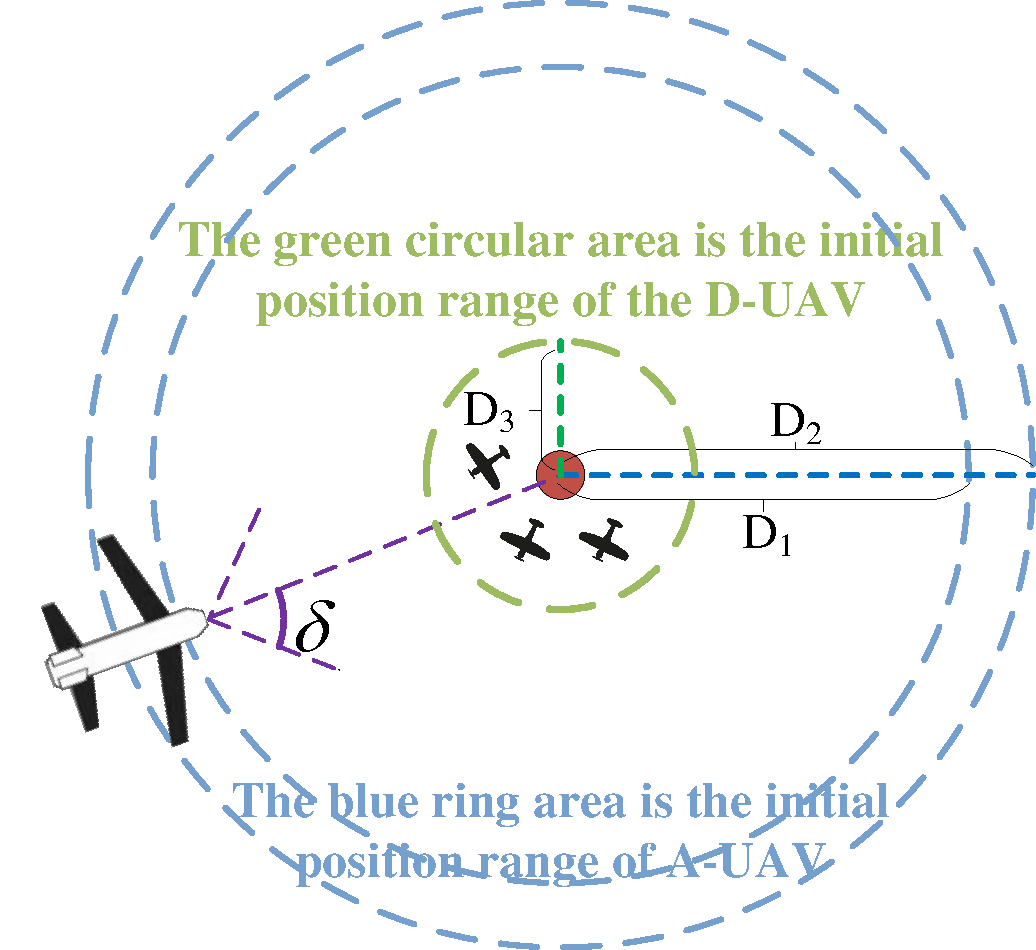
\includegraphics[width=3.0in]{chushi01.pdf}
\caption{Simulation environment configuration for training.}
\label{chushi}
\end{figure}

A representative scenario of 20 $D_{\text{UAV}}$ versus 8 $A_{\text{UAV}}$ is considered, with $D_1=100$\,m,
$D_2=1500$\,m, and $D_3=1600$\,m.
Table~\ref{chushicanshu} summarizes the UAV kinematic parameters.

\begin{table*}[!t]
\centering
\caption{UAV Parameters for Attackers and Defenders}
\label{chushicanshu}
\renewcommand{\arraystretch}{1.6}
\begin{tabular}{ccccc}
\hline\hline
 & Initial position $(x,y)$ & Initial velocity $V$ & Initial heading $\gamma$ & Maneuverability $(n_x,n_y,V)$ \\ \hline
$D_{\text{UAV}}$ & $r\sim U[0,D_3]$, $\theta\sim U[0,2\pi]$ & $V_D\sim U[10,40]$\,m/s & $\gamma_D\sim U[0,2\pi]$ & $n_x\in[-0.1g,1g]$, $n_y\in[-1g,1g]$ \\
$A_{\text{UAV}}$ & $r\sim U[D_1,D_2]$, $\theta\sim U[0,2\pi]$ & $V_A\sim U[10,40]$\,m/s & $\gamma_A\sim U[q_A-30^\circ,q_A+30^\circ]$ & $n_x=0$, $n_y\in[-1g,1g]$ \\ \hline
\end{tabular}
\end{table*}

Two dynamic engagement scenarios are designed to evaluate cooperative guidance performance.
The scenario configurations are listed in Table~\ref{changjingqingkuang}.

\begin{table}[!t]
\centering
\renewcommand{\arraystretch}{1.4}
\caption{Combat Scenario Settings}
\label{changjingqingkuang}
\begin{tabular}{cccc}
\hline\hline
 & $N_{D\text{-UAV}}$ & $N_{A\text{-UAV}}$ & $A_{\text{UAV}}$ Strategy \\ \hline
Case 1 & 20 & 8 & Hybrid Evasion \\
Case 2 & 20 & 8 & Sinusoidal Maneuver \\ \hline
\end{tabular}
\end{table}




\subsection{Target Assignment Performance and Spatial Topology}
\label{subsec:assignment_results}

To evaluate the IDBO algorithm, it is benchmarked against PSO, GWO, SSA, BOA, and standard DBO. 

Fig.~\ref{fig:convergence} illustrates the statistical performance in terms of average cost convergence over iterations. IDBO significantly outperforms the baselines, reaching the lowest steady-state cost within 100~iterations. \begin{figure}[!ht] 
\centering 
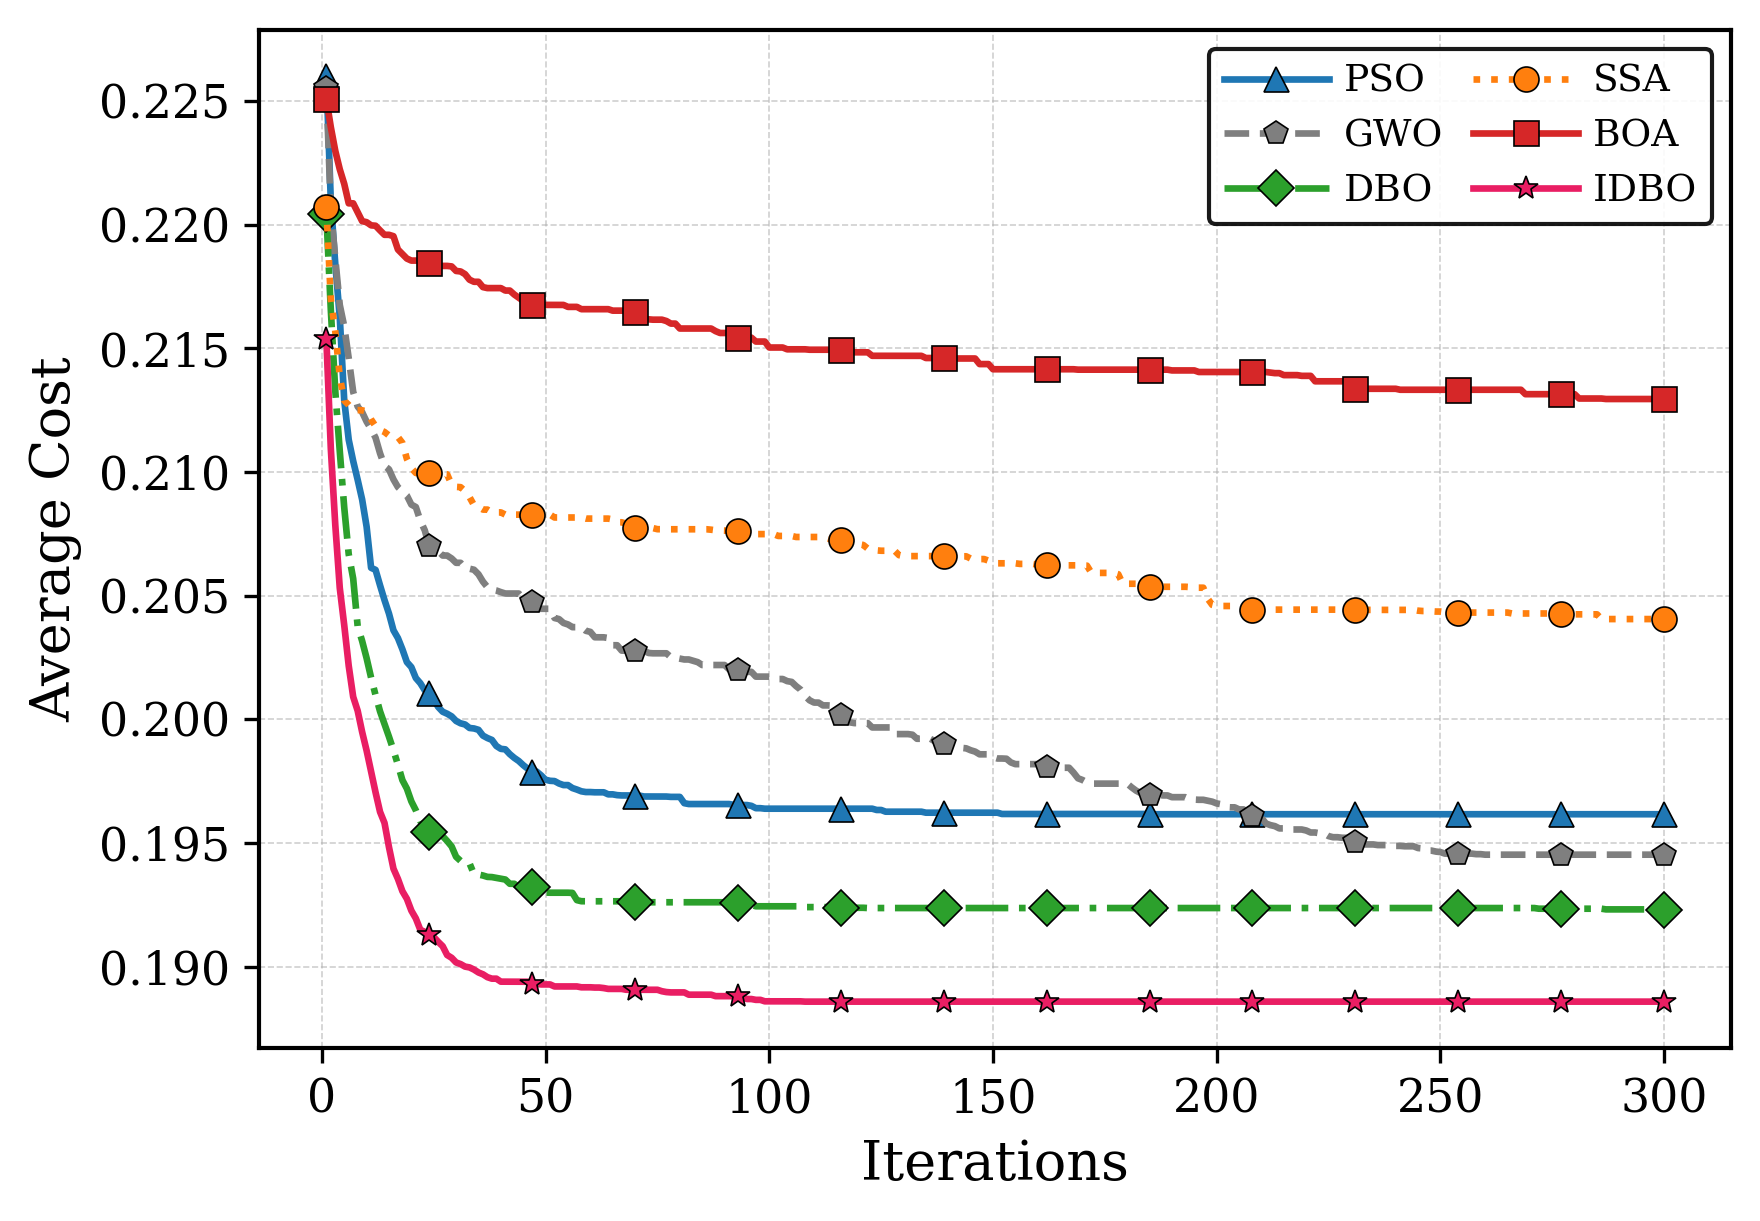
\includegraphics[width=3.25in]{convergence.png} 
\caption{Average cost convergence over iterations for target assignment algorithms.} 
\label{fig:convergence} 
\end{figure}

Furthermore, the violin plot in Fig.~\ref{fig:violin} evaluates the algorithmic robustness across multiple independent runs. It shows IDBO's compact distribution at the lowest median cost, highlighting its superior stability and consistency compared to the other heuristic methods.

\begin{figure}[!ht] 
\centering 
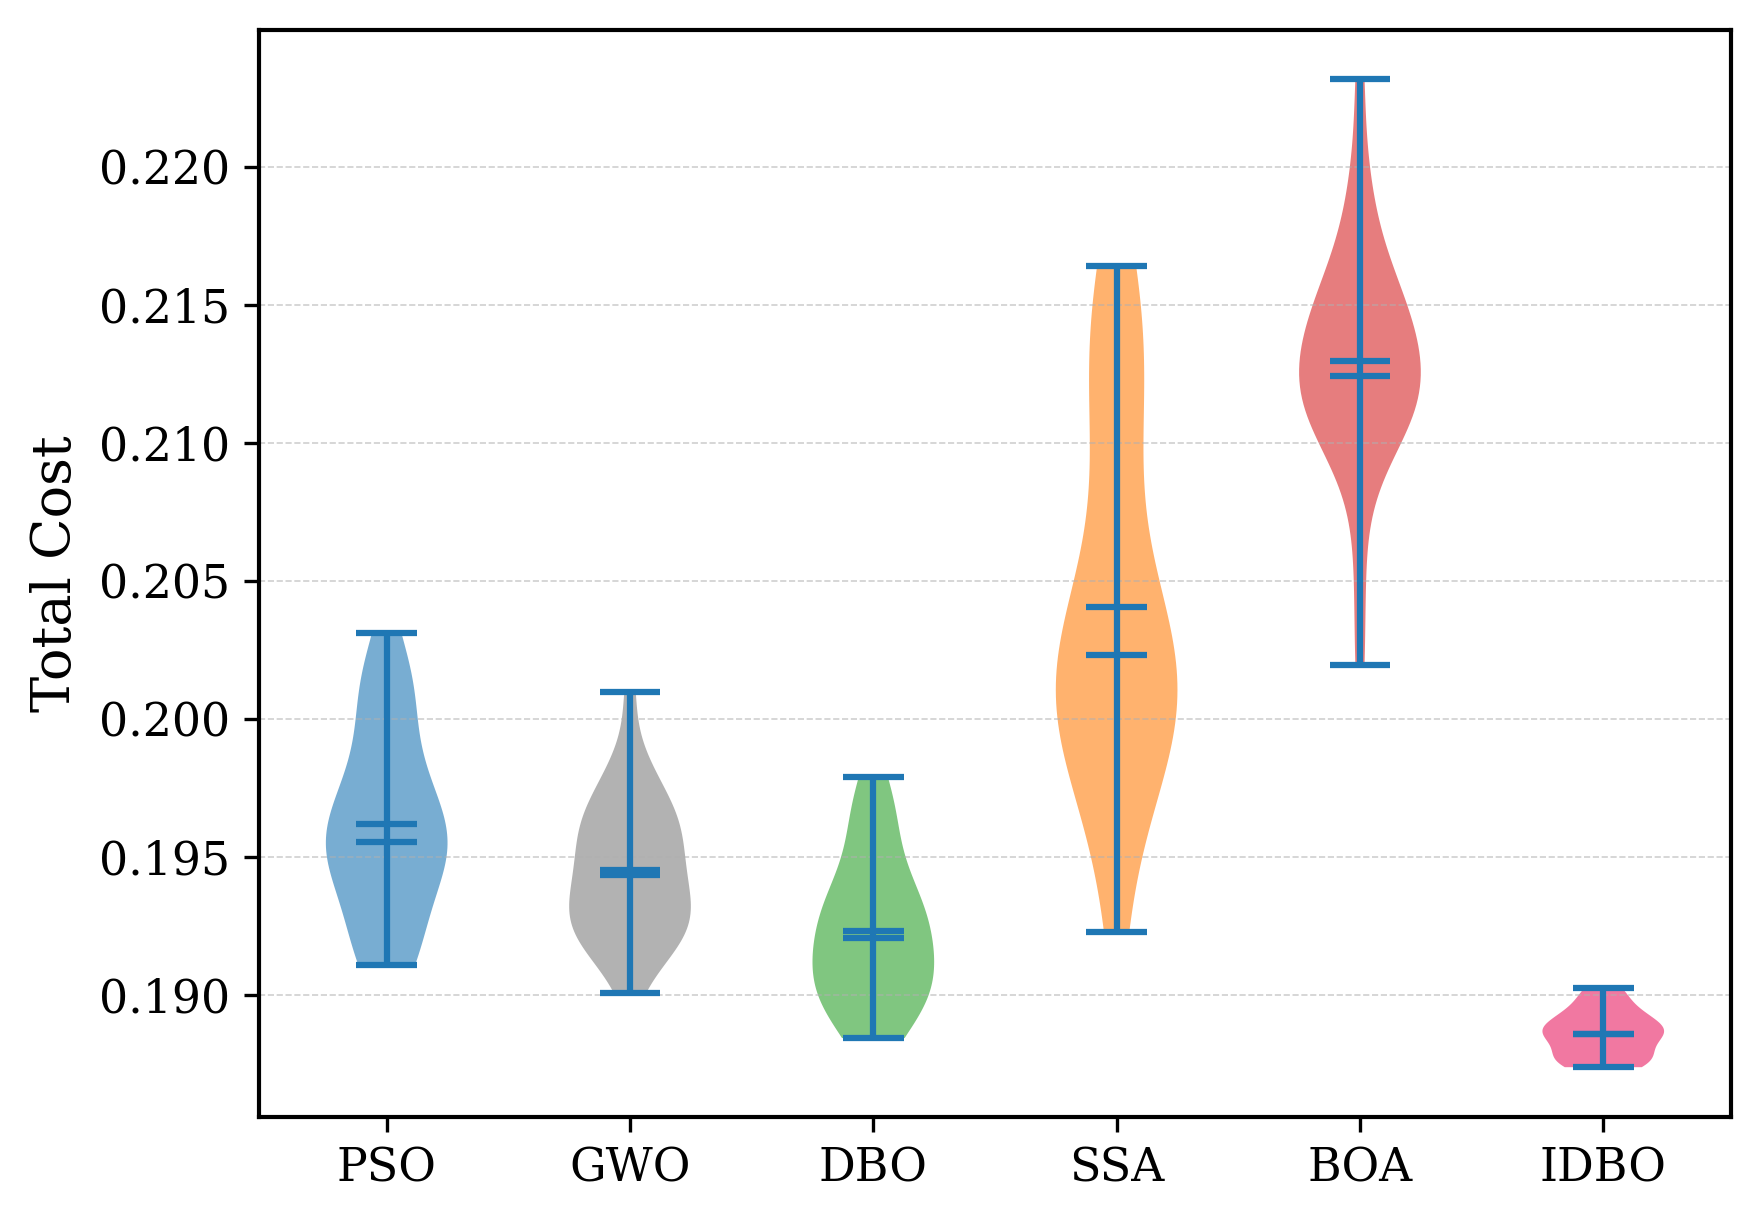
\includegraphics[width=3.2in]{violin.png} 
\caption{Violin plot of total cost distribution evaluating algorithm robustness.} 
\label{fig:violin} 
\end{figure}

The optimal assignment mapping generated by the algorithm is visualized in Fig.~\ref{fig:assignment_topology}. Attackers $A_1$--$A_4$ are each allocated three defenders, while $A_5$--$A_8$ are intercepted by two defenders each, perfectly respecting the per-target capacity constraint $L_{\max}$ and ensuring sufficient numerical superiority for cooperative strikes.

\begin{figure}[!ht]
\centering
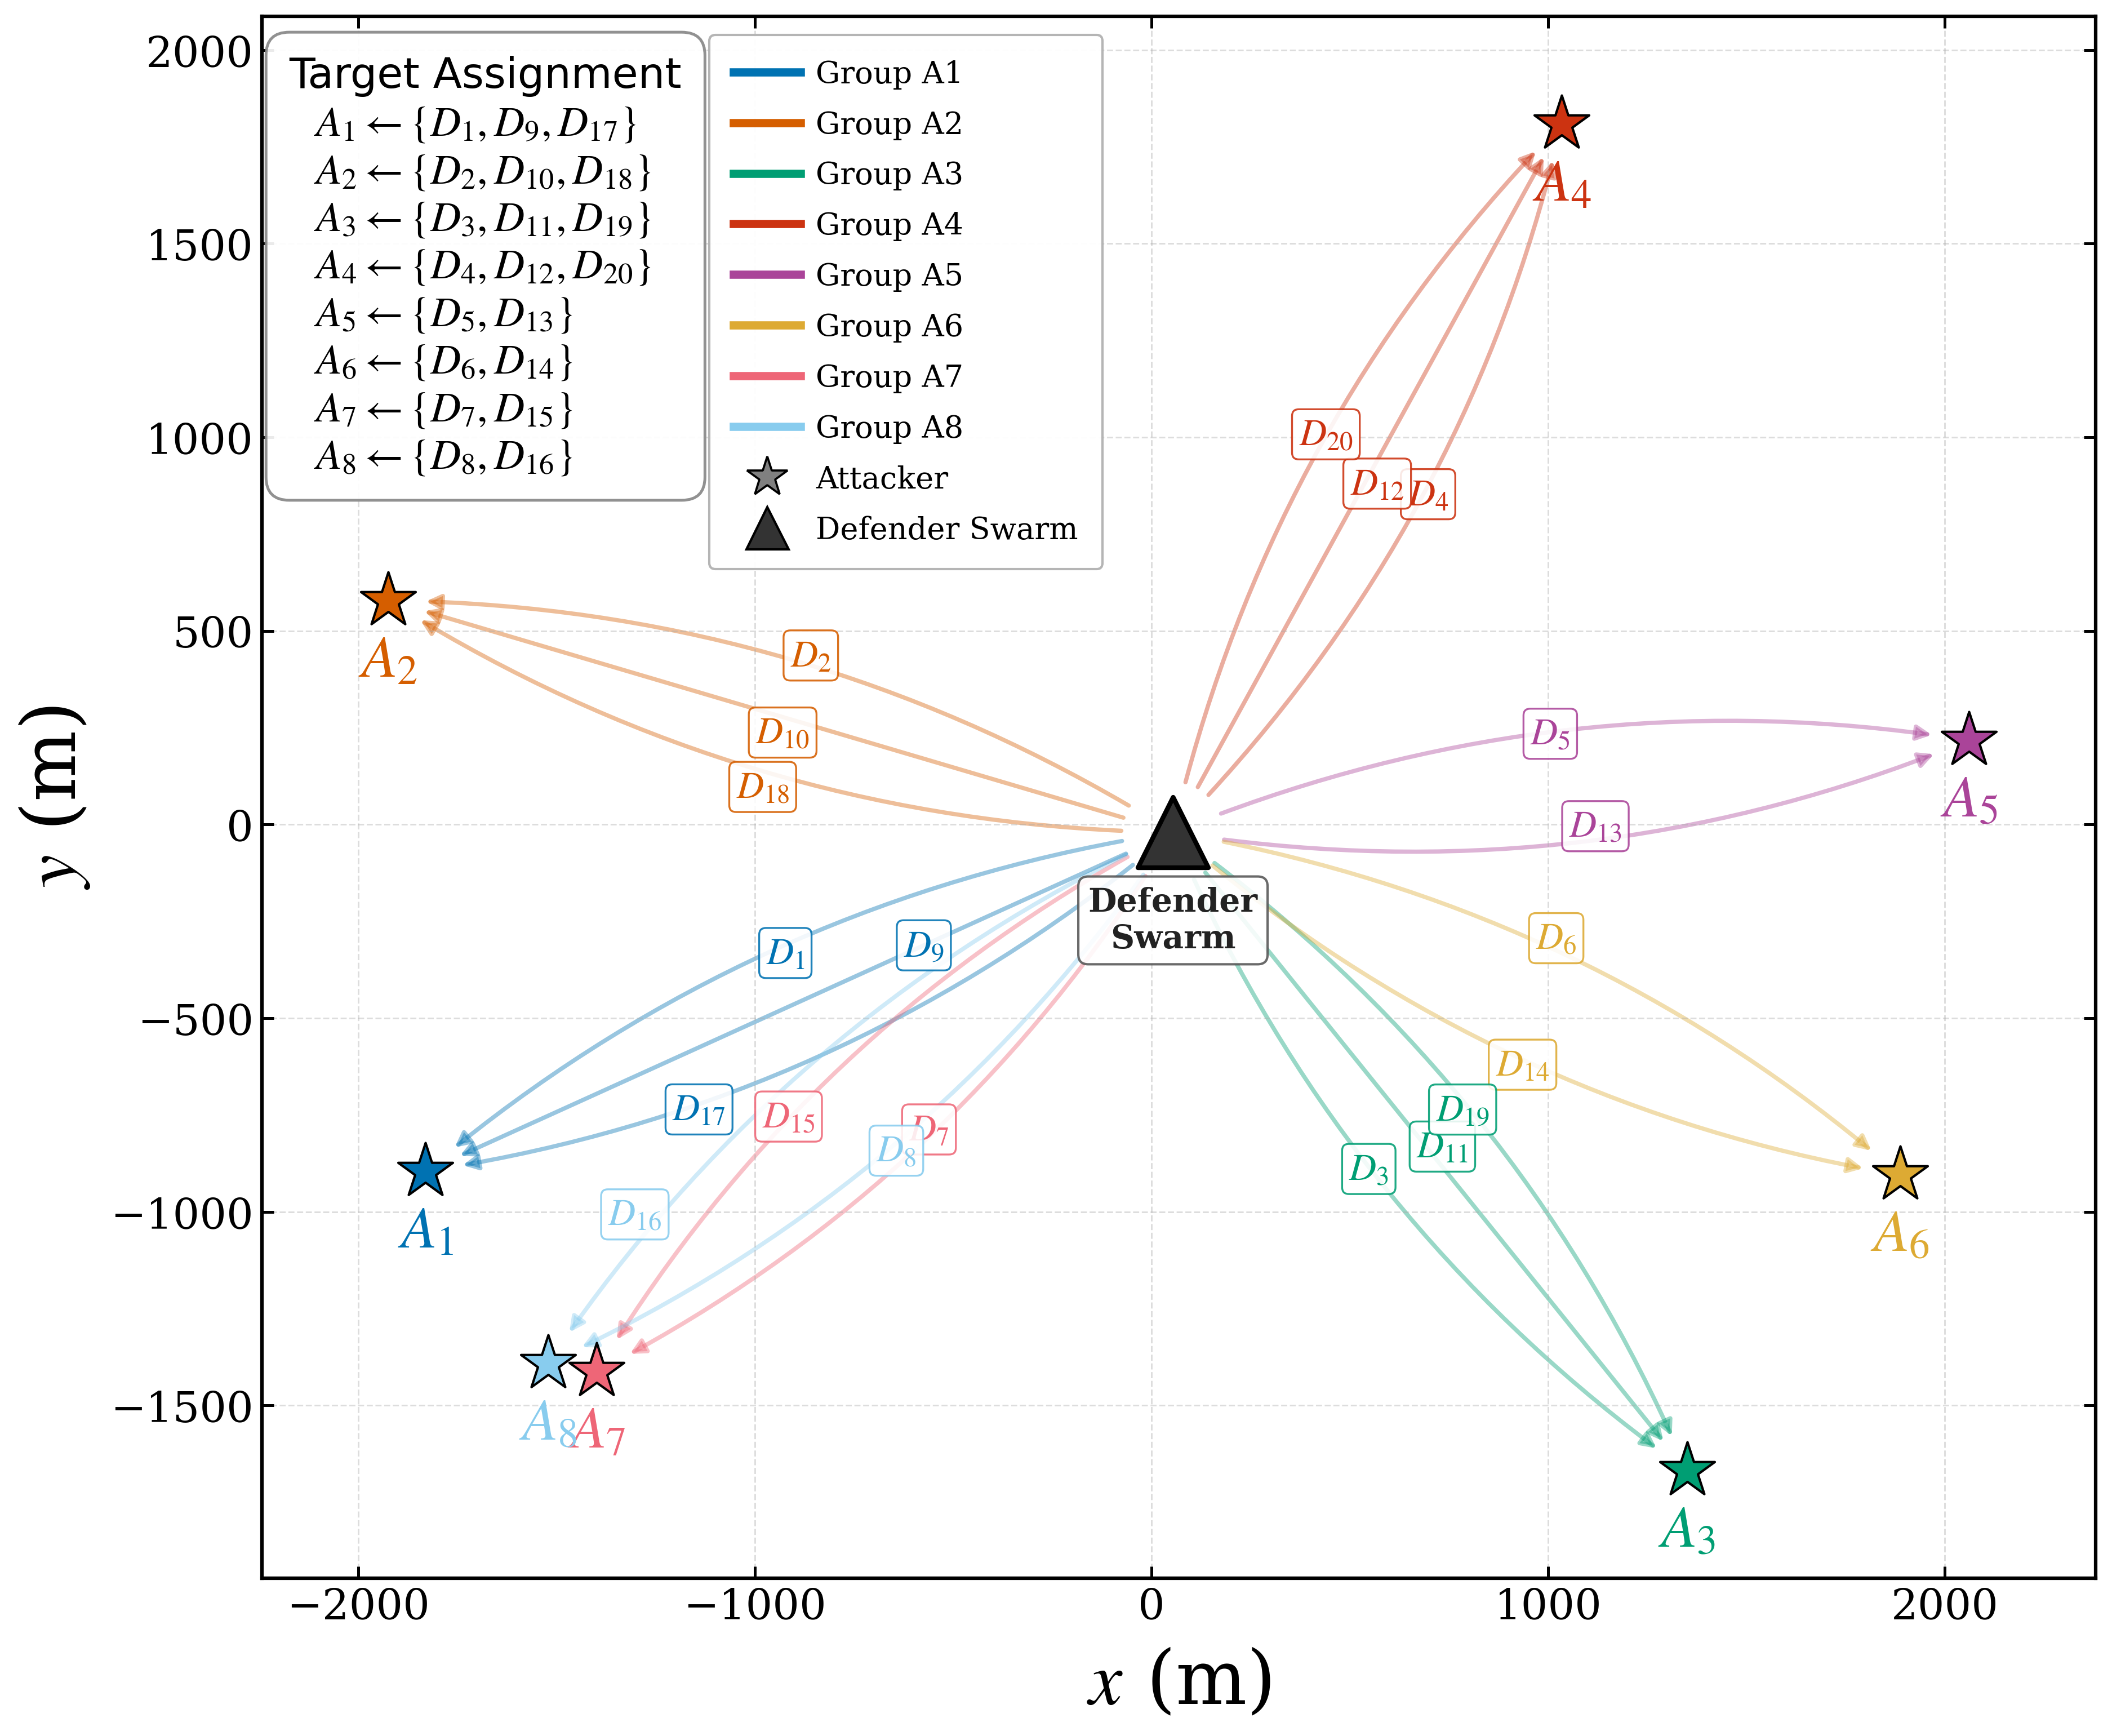
\includegraphics[width=3.2in]{target_assignment_topology.png}
\caption{Visualized spatial topology of the target assignment results.}
\label{fig:assignment_topology}
\end{figure}








\subsection{RL Model Training and Convergence Analysis}
\label{subsec:training}

To evaluate the learning efficiency and robustness of the proposed ART-MAPPO, comparative training experiments were conducted against standard MAPPO, IPPO, IA2C, and IQL. All models were trained over 10,000 episodes with a maximum horizon of 25 steps per episode. To ensure statistical significance and eliminate the bias of favorable network initialization, all learning curves in Fig.~\ref{fig:training_convergence} are averaged across 5 independent random seeds, with the shaded regions denoting the standard deviation.

As illustrated in Fig.~\ref{fig:training_convergence}(a), ART-MAPPO demonstrates a superior learning paradigm, achieving the highest asymptotic normalized reward of $8.97 \pm 0.64$ (averaged over the final 500 episodes). This represents a notable performance improvement of 8.2\%, 12.3\%, 14.4\%, and 29.8\% over IQL, MAPPO, IPPO, and IA2C, respectively. The advantage of ART-MAPPO is particularly pronounced during the intermediate training phase. By episode 4,000, ART-MAPPO establishes a significant performance leap, outperforming standard MAPPO by 43.6\% and IQL by 16.6\%, highlighting its ability to rapidly escape local optima early in the training process.

Furthermore, the proposed method exhibits accelerated convergence alongside enhanced training stability. When evaluated on a 100-episode smoothed curve, ART-MAPPO reaches 90\% of its optimal asymptotic performance by episode 5,591. In contrast, the most competitive baseline, IQL, requires 6,477 episodes (a 13.7\% delay), while standard MAPPO lags significantly, requiring 7,654 episodes. Regarding algorithmic stability, ART-MAPPO maintains a tight variance across random seeds ($\sigma = 0.64$), whereas standard MAPPO exhibits a standard deviation of 1.34 (approximately twice as large). This confirms that the proposed enhancements effectively mitigate the high-variance gradient updates typical in multi-agent policy-based methods.

These macroscopic performance gains are directly supported by the network-level metrics. The critic loss (Fig.~\ref{fig:training_convergence}(b)) of ART-MAPPO converges to the lowest steady-state error with minimal oscillation, a direct consequence of the dual-clip mechanism and adaptive KL penalty. Concurrently, the policy entropy (Fig.~\ref{fig:training_convergence}(c)) demonstrates an optimal, gradual decay trajectory, validating that the trust-modulated exploration mechanism successfully balances early-stage extensive state-space exploration with late-stage strict policy exploitation.

\begin{figure}[!t]
\centering
\subfloat[Training Reward]{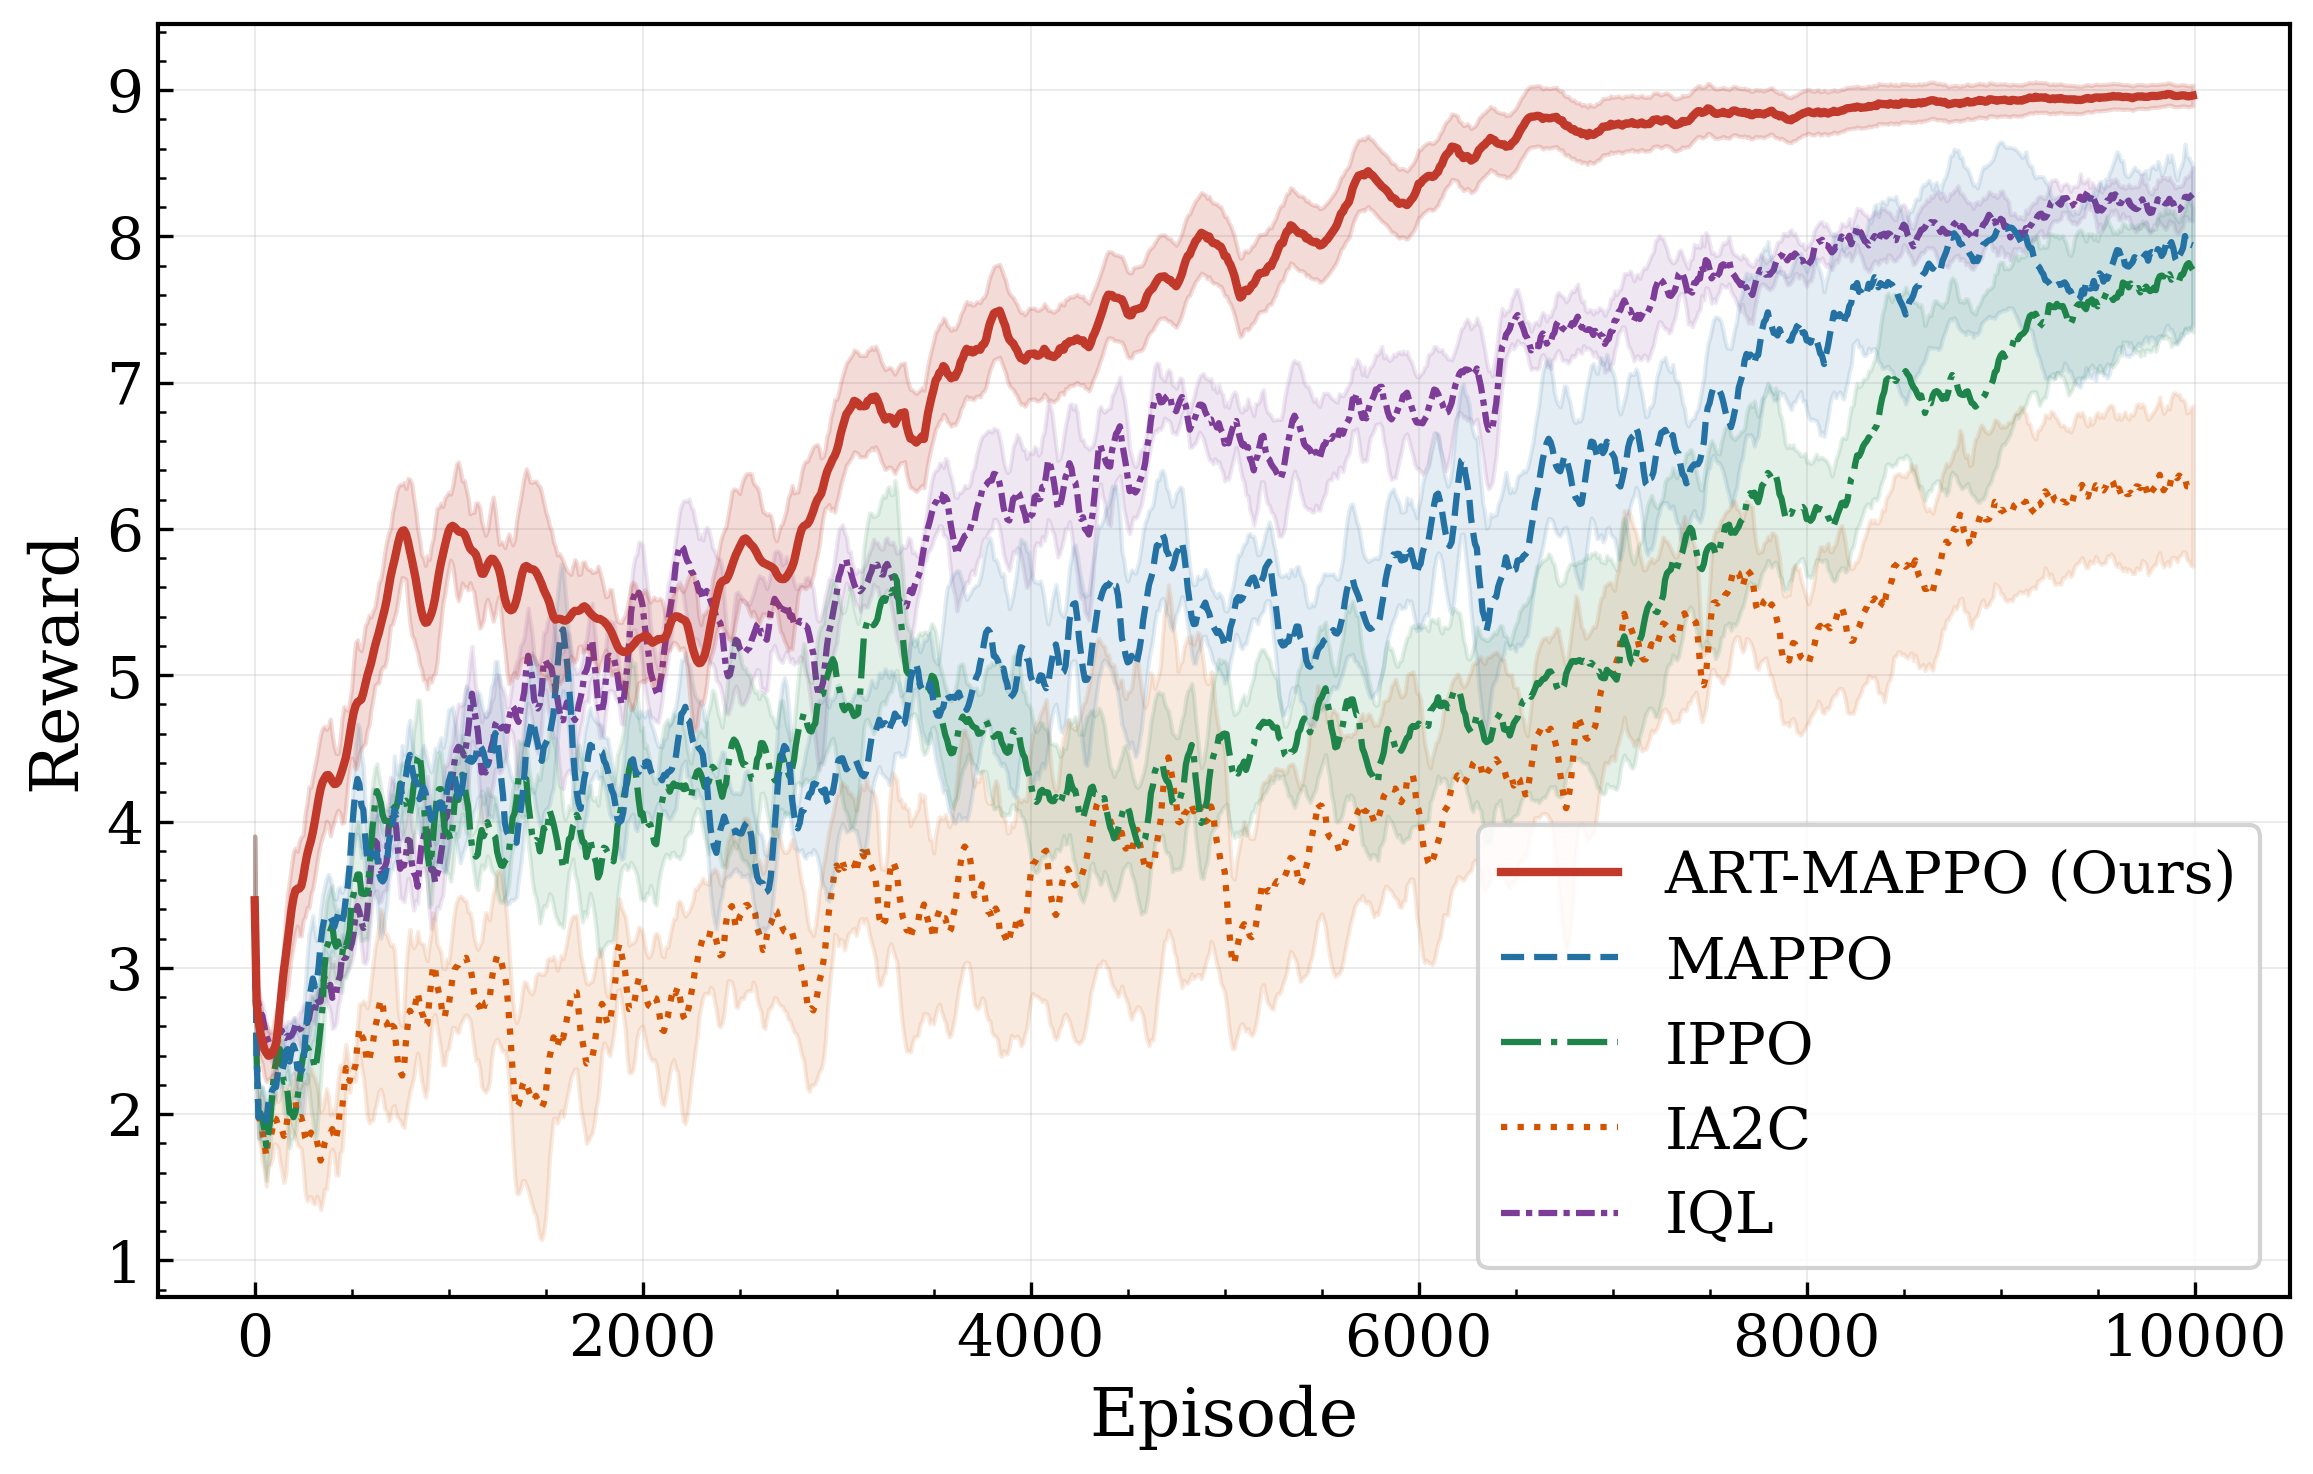
\includegraphics[width=3.0in]{fig_a_reward.png}}
\hfill
\subfloat[Critic Loss]{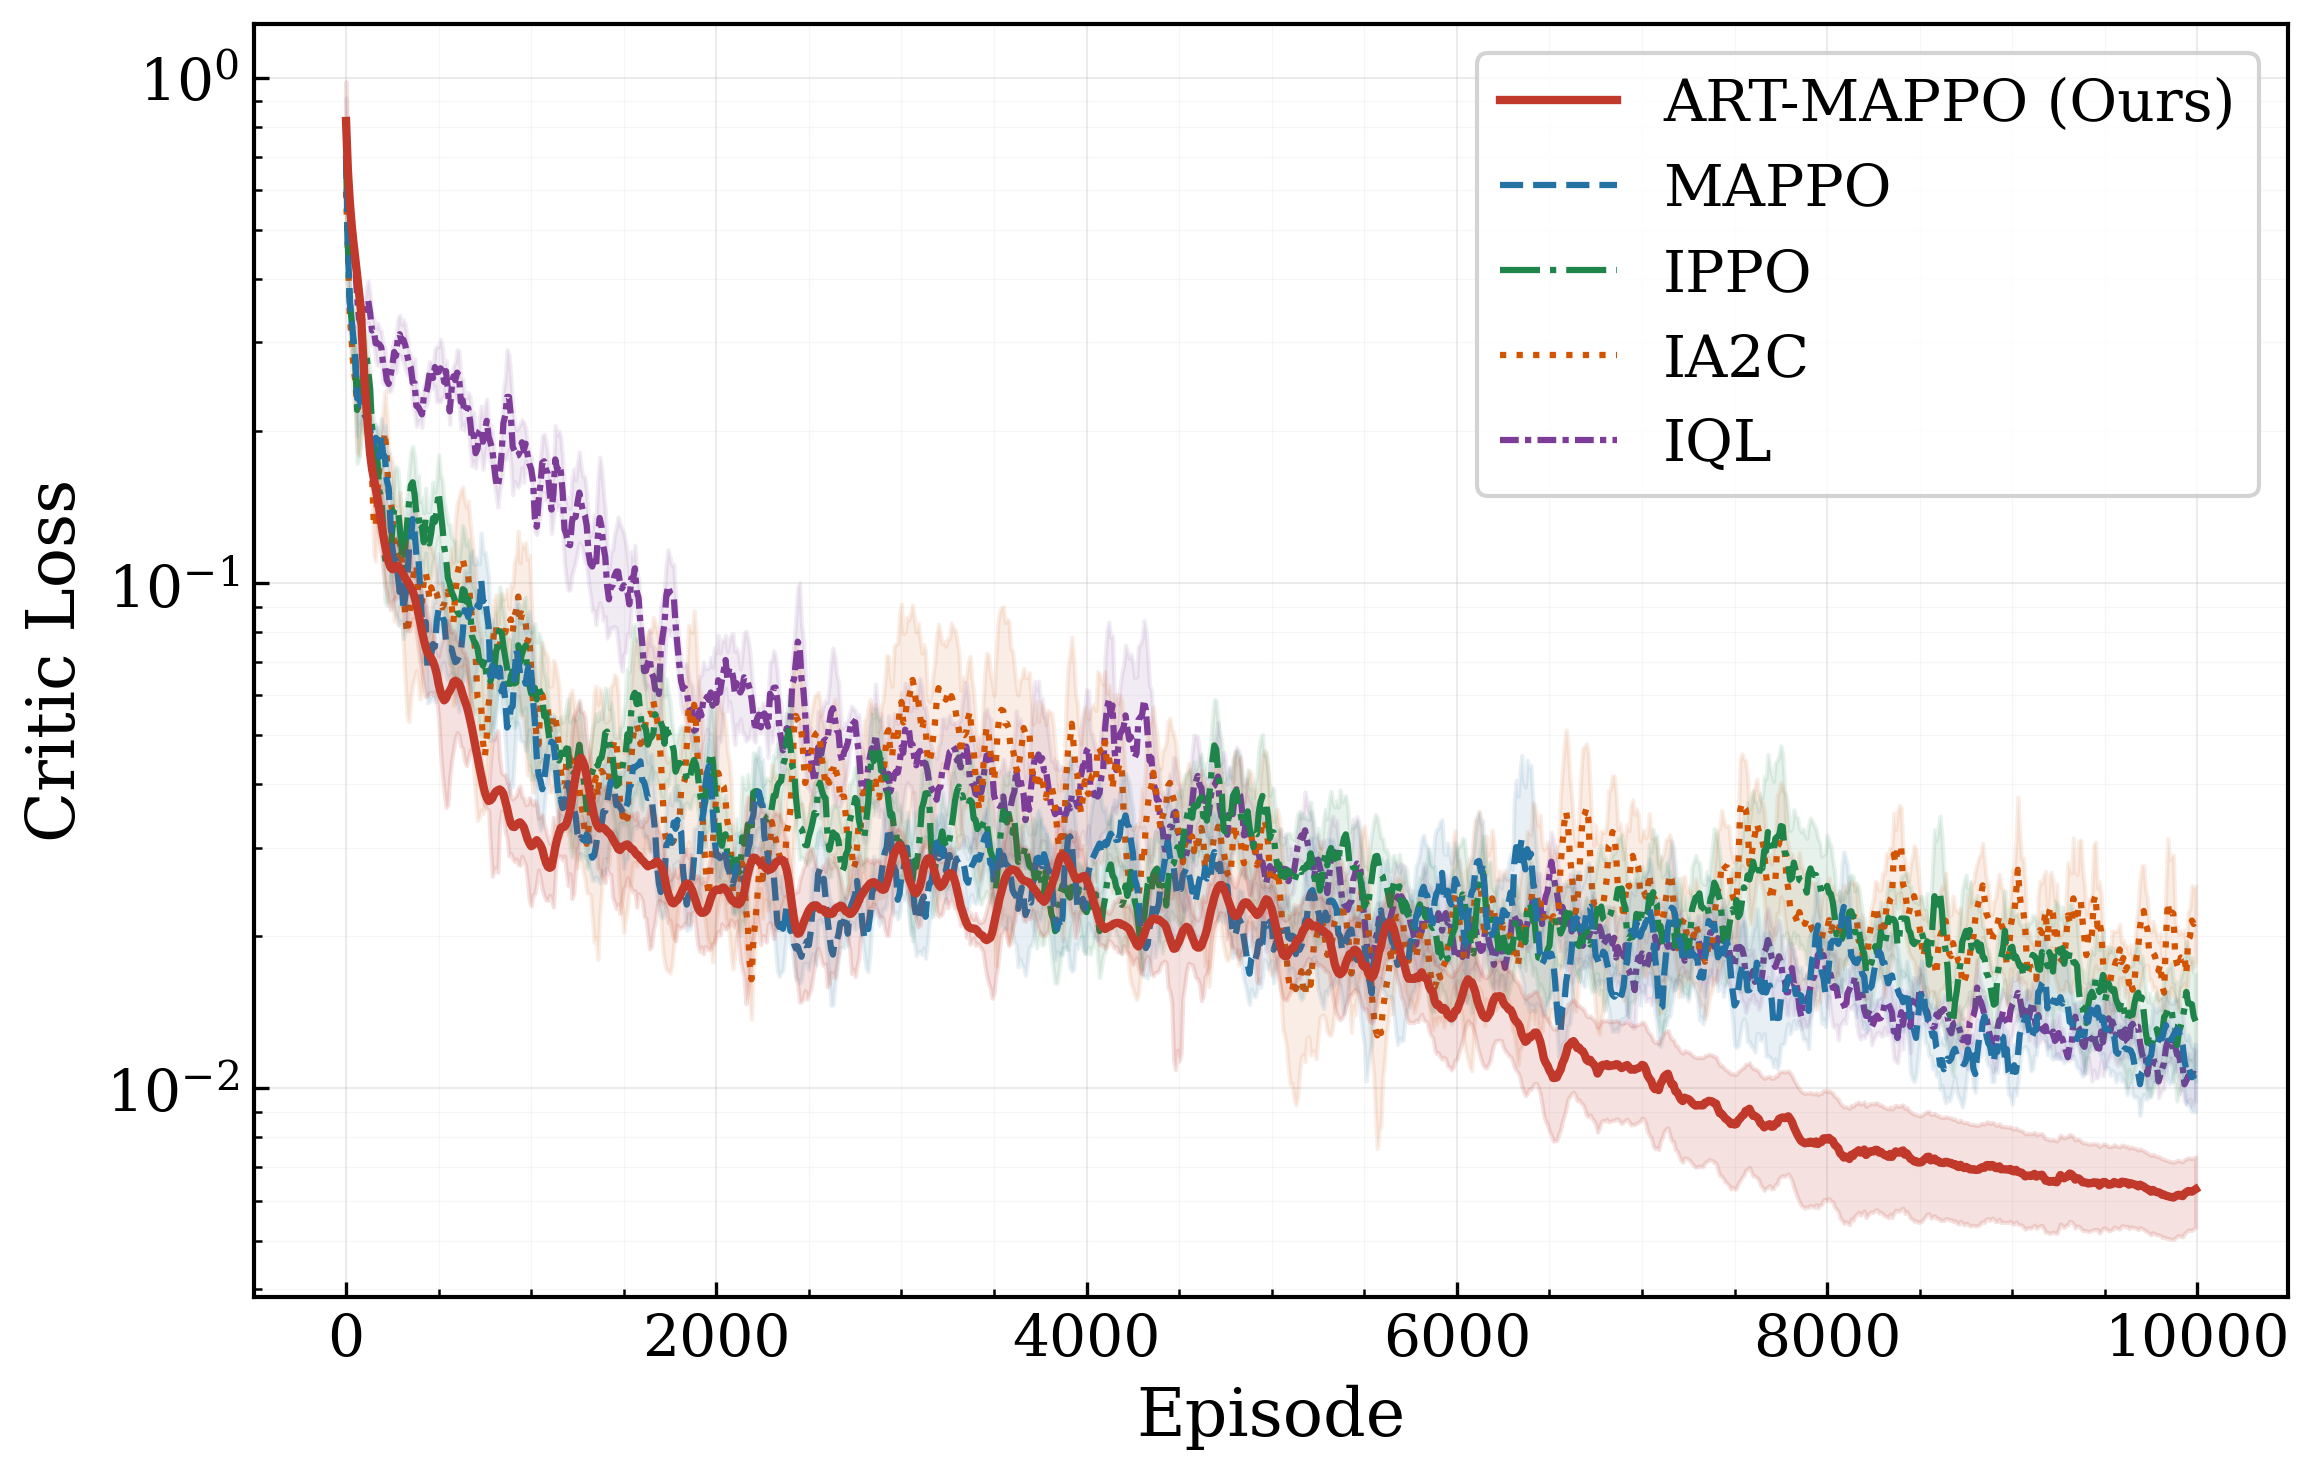
\includegraphics[width=3.0in]{fig_b_critic_loss.png}}
\hfill
\subfloat[Policy Entropy]{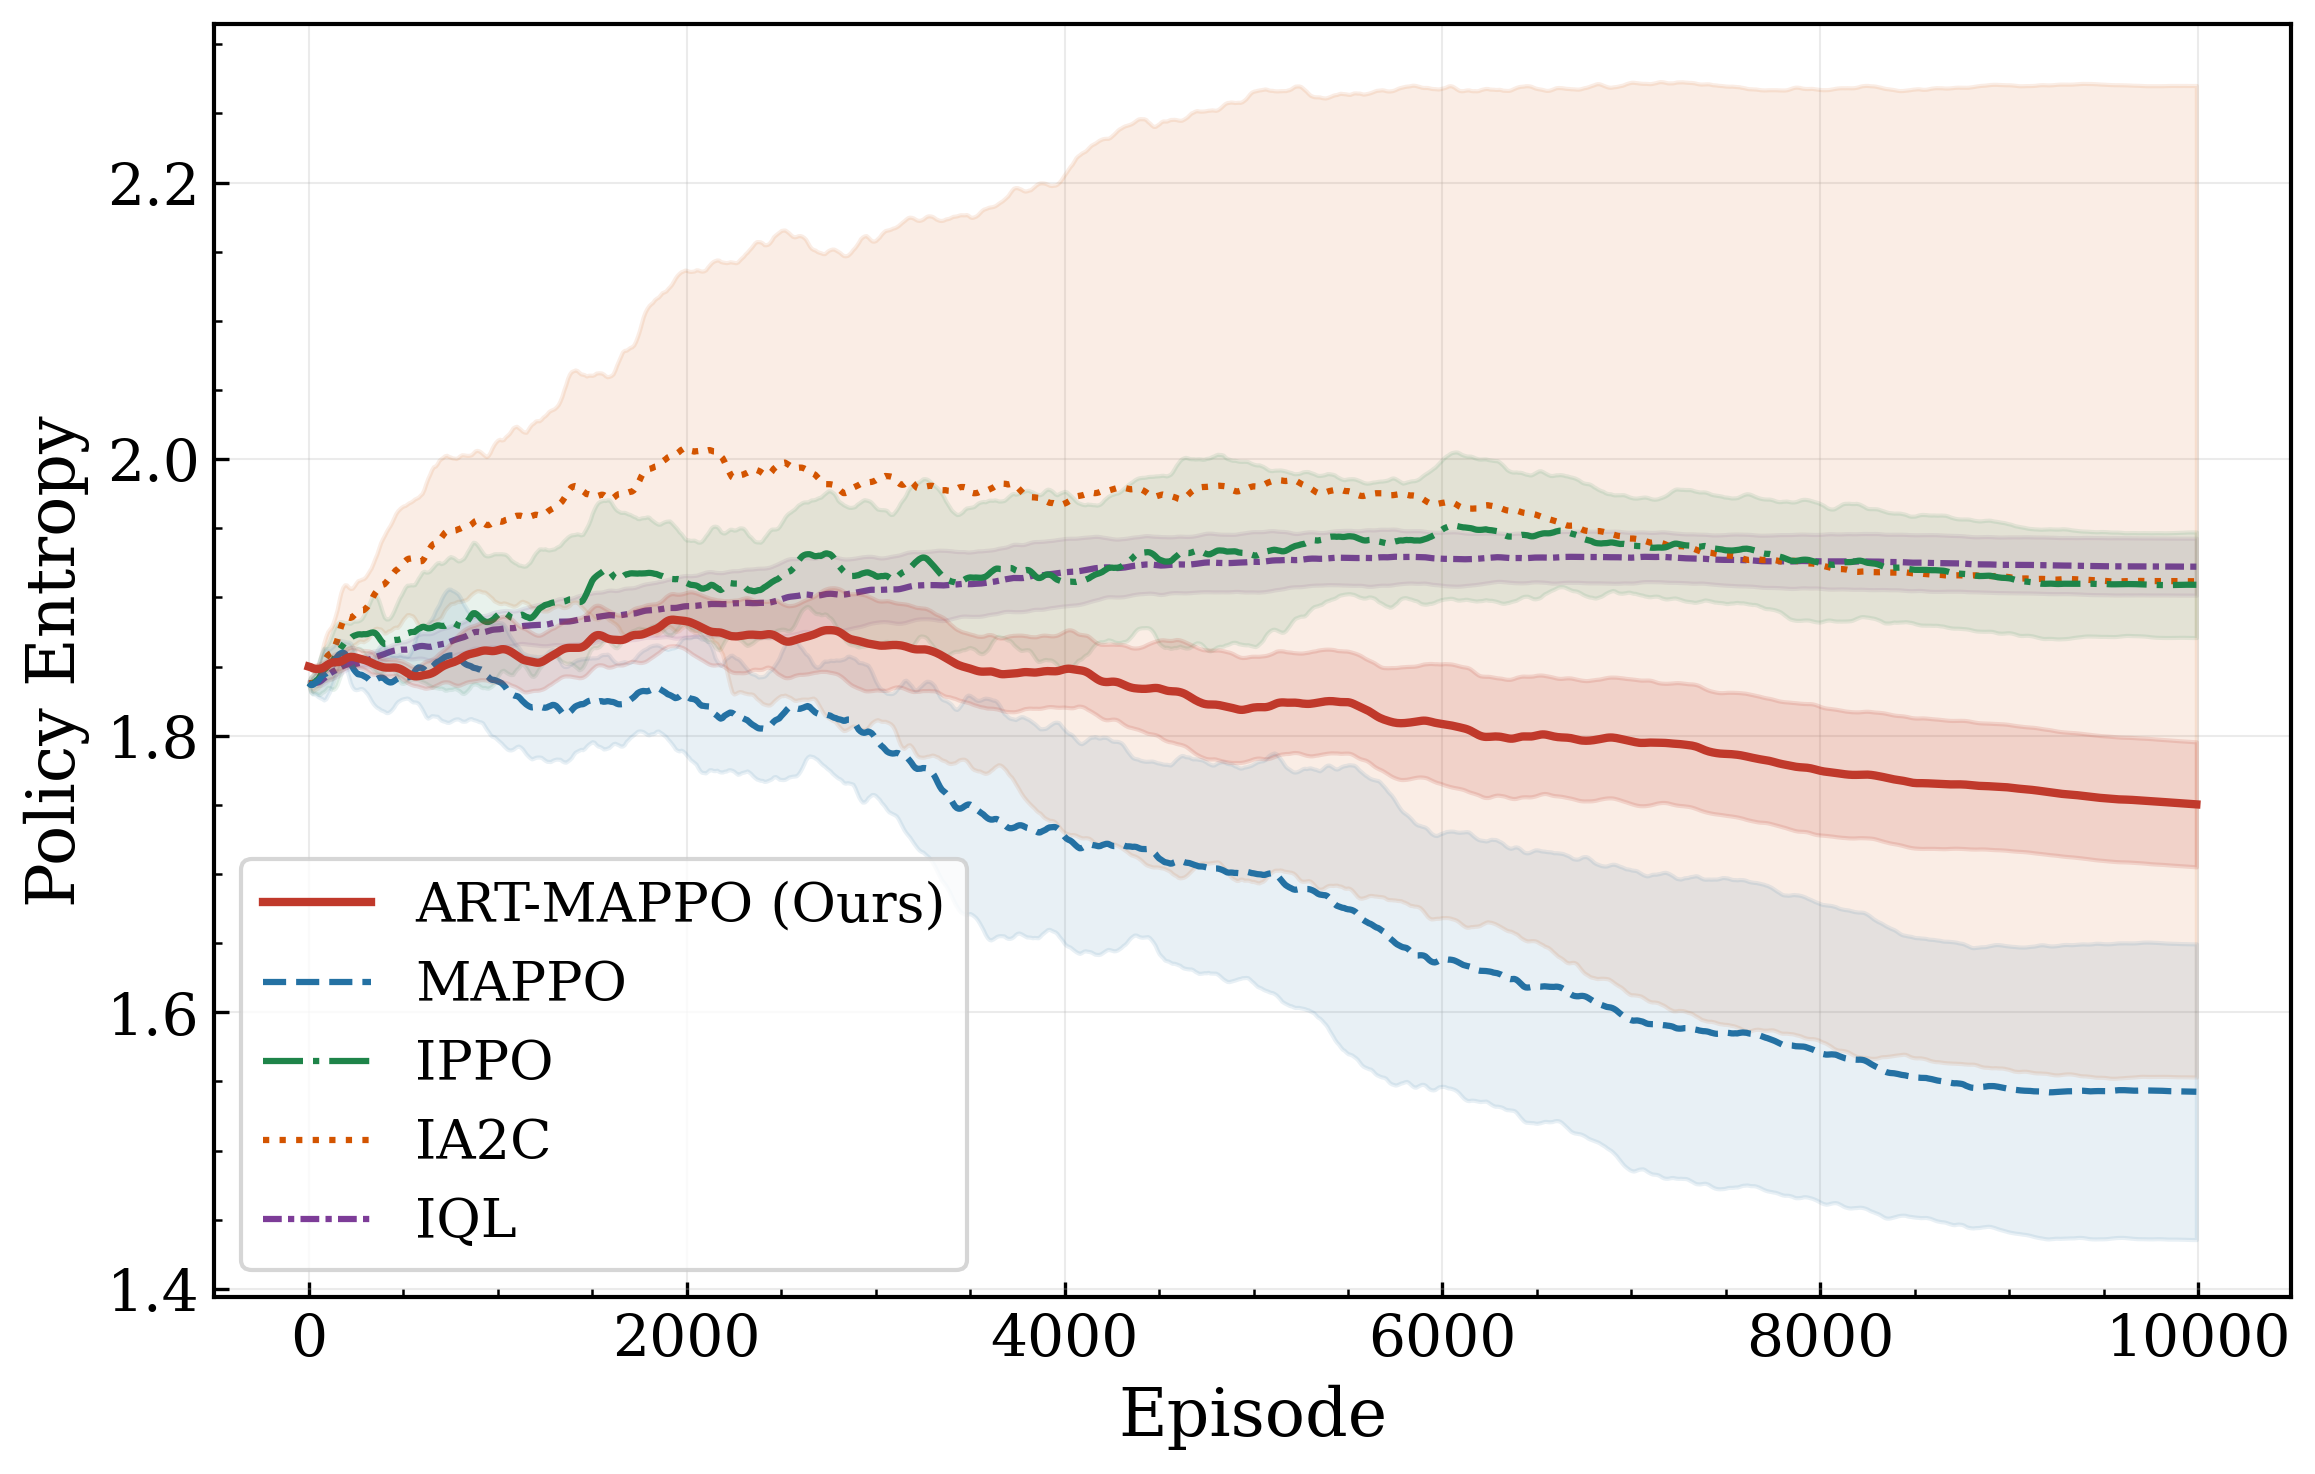
\includegraphics[width=3.0in]{fig_c_entropy.png}}
\caption{Comparative training curves of ART-MAPPO and baseline algorithms over 10,000 episodes. Solid lines and shaded regions represent the mean and standard deviation across 5 independent random seeds, respectively. Notably, ART-MAPPO achieves the highest asymptotic reward (+12.3\% over standard MAPPO) and the fastest convergence rate (reaching 90\% optimality by episode 5,591), while demonstrating significantly enhanced training stability.}
\label{fig:training_convergence}
\end{figure}


%%%%-------------------------------------------------------------------------------------------

\subsection{Cooperative Interception against Maneuvering Targets}
\label{subsec:cases}

Based on the optimal assignment topology, we evaluate the terminal cooperative guidance
performance against two maneuvering scenarios, each benchmarked against classical PN.







\subsubsection{Case~1: Interception against Evasive Maneuvering Targets}

In this scenario, the attacking UAVs ($A_{\text{UAV}}$) initially execute a constant-$g$ evasive maneuver and transition to proportional navigation (PN) guidance after 15\,s. The defending swarm is tasked with neutralizing these highly dynamic threats utilizing the pre-computed assignment topology.

Fig.~\ref{fig:case1_mappo_traj} illustrates the 2D engagement trajectories generated by the proposed ART-MAPPO algorithm. Guided by the intelligent policy, the defending swarm effectively divides into eight coordinated combat units. Despite the evasive maneuvers of the targets, ART-MAPPO generates remarkably smooth and direct pursuit curves, enabling all interceptors to successfully converge on their respective targets without unnecessary detours.

\begin{figure}[!ht]
\centering
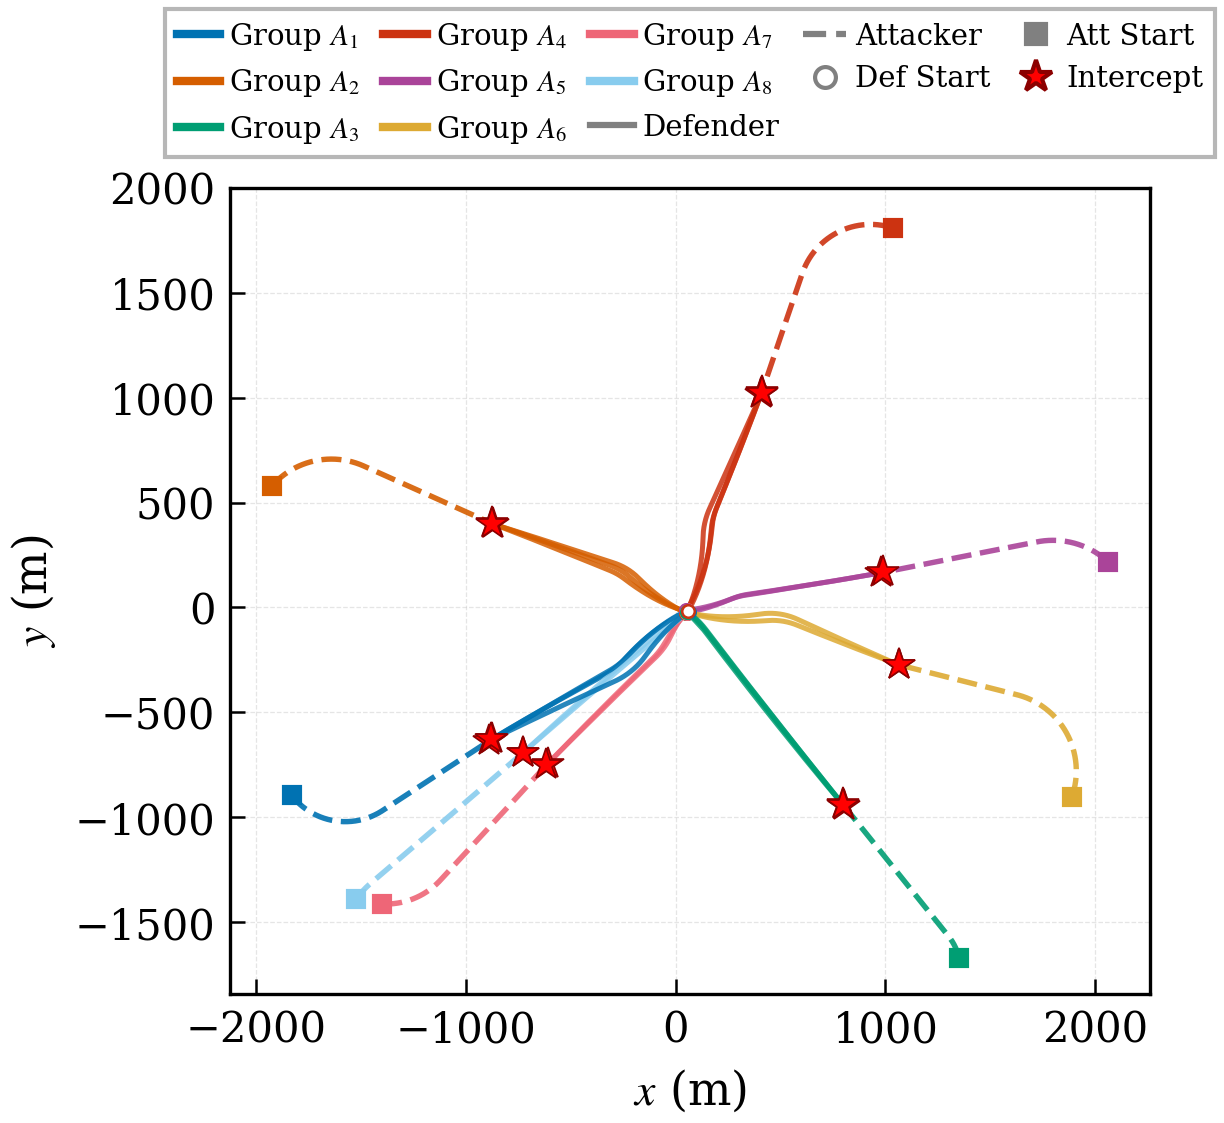
\includegraphics[width=3.2in]{mappo_nopn_trajectory.png}
\caption{Engagement trajectories of the defending swarm using ART-MAPPO in Case~1.}
\label{fig:case1_mappo_traj}
\end{figure}

To deeply analyze the operational efficiency and constraint adherence of the proposed method, Fig.~\ref{fig:case1_mappo_kine} presents the comprehensive kinematic and control profiles of ART-MAPPO. Most critically, the normal acceleration ($n_y$) profile in Fig.~\ref{fig:case1_mappo_kine}(a) highlights the safety and robustness of the learned policy: ART-MAPPO strictly bounds its lateral overload within the physical $\pm1$\,g limit throughout the entire mid-course and terminal phases, completely avoiding the risk of actuator saturation. Furthermore, the heading angles smoothly adjust to the optimal collision course (Fig.~\ref{fig:case1_mappo_kine}(b)). As shown in the velocity ($V_D$) and axial acceleration ($n_x$) profiles (Fig.~\ref{fig:case1_mappo_kine}(c) and (d)), ART-MAPPO actively manages its forward energy, commanding maximum axial acceleration early in the engagement to rapidly reach the speed limit of 40\,m/s. This intelligent energy management dramatically minimizes the overall interception duration.

\begin{figure}[!ht]
\centering

\includegraphics[width=3.0in]{standalone_duav_legend.png}
\subfloat[Normal acceleration $n_y$]{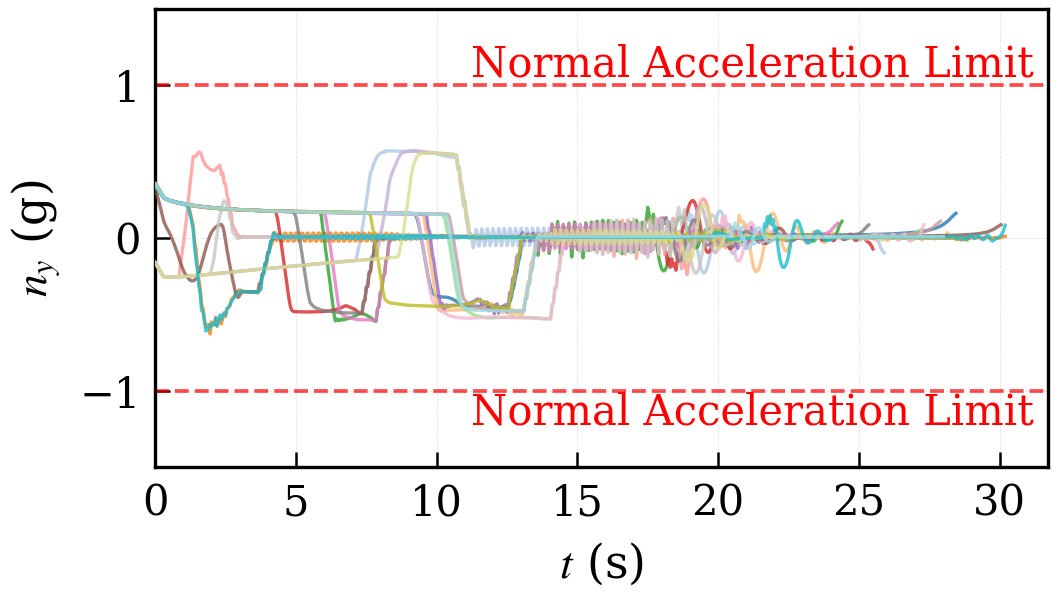
\includegraphics[width=3.0in]{mappo_nopn_ny.png}}
\hfil
\subfloat[Heading angle $\gamma_D$]{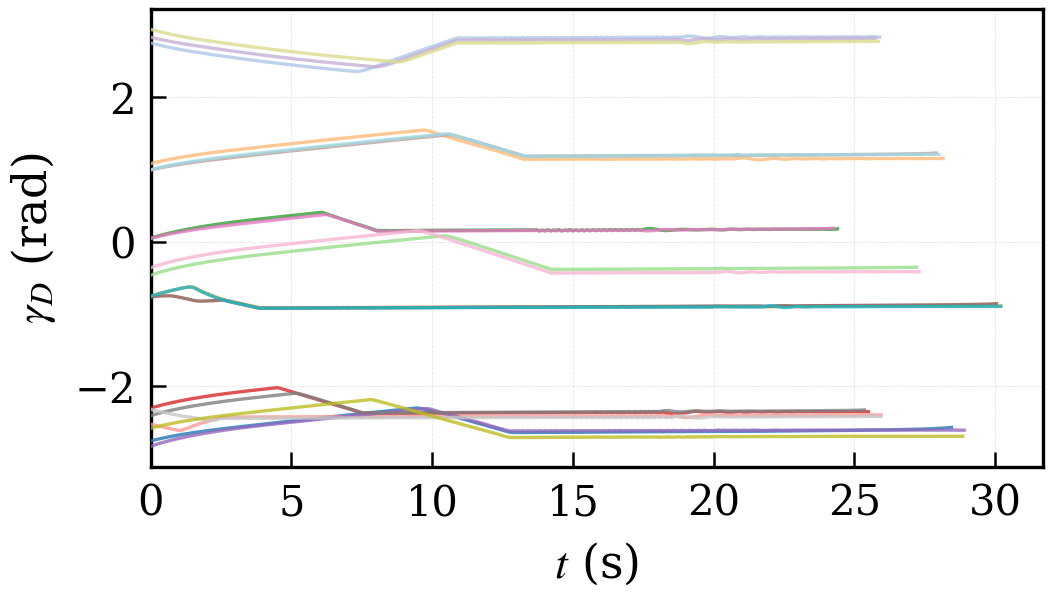
\includegraphics[width=3.0in]{mappo_nopn_heading.png}}
\hfil
\subfloat[Velocity $V_D$]{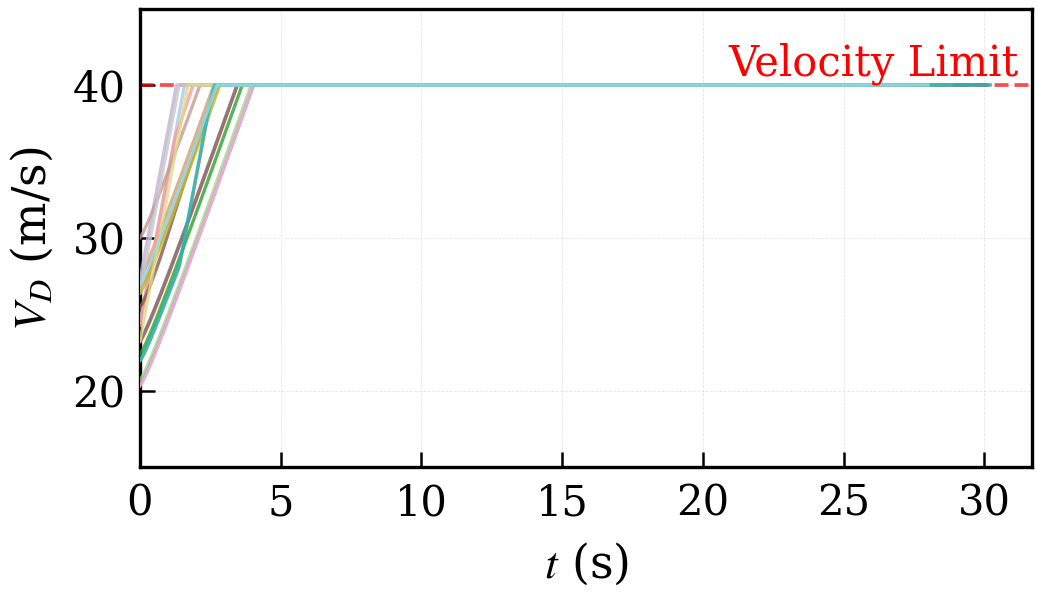
\includegraphics[width=3.0in]{mappo_nopn_velocity.png}}
\hfil
\subfloat[Axial acceleration $n_x$]{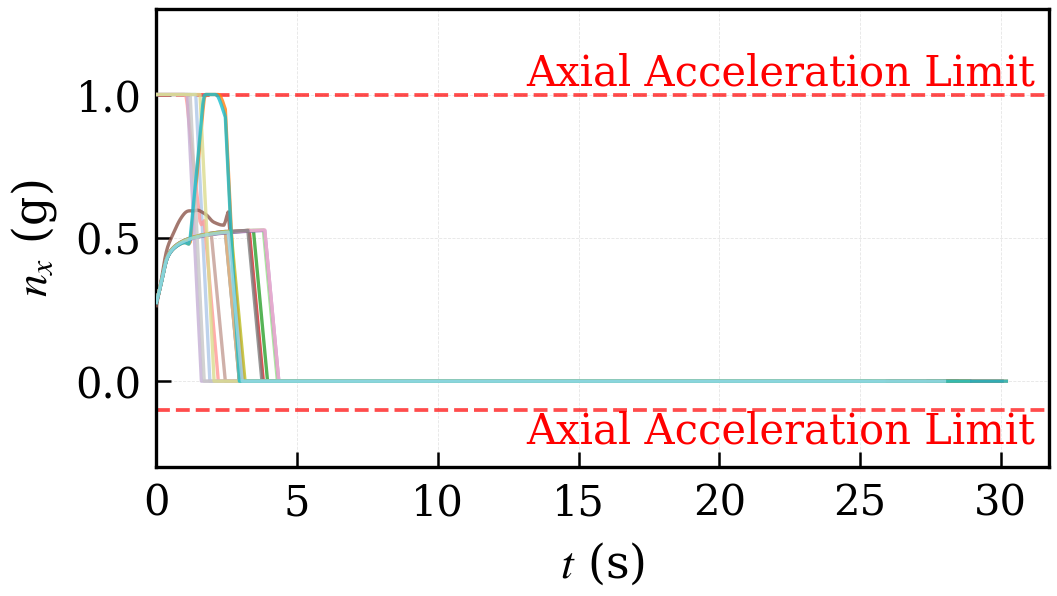
\includegraphics[width=3.0in]{mappo_nopn_nx.png}}
\vspace{0pt}
\caption{Kinematic and control effort profiles of ART-MAPPO for Case~1. The algorithm successfully maximizes closing speed while strictly adhering to the $\pm1$\,g normal overload constraint.}
\label{fig:case1_mappo_kine}
\end{figure}

In stark contrast, the performance of the baseline PN guidance is presented in Fig.~\ref{fig:case1_pn_traj} and Fig.~\ref{fig:case1_pn_kine}. While PN eventually intercepts the targets (Fig.~\ref{fig:case1_pn_traj}), its purely reactive nature leads to a highly inefficient pursuit strategy. As clearly depicted in Fig.~\ref{fig:case1_pn_kine}(a), the normal acceleration ($n_y$) of PN drastically diverges, severely violating the $\pm1$\,g physical limit because the algorithm lacks predictive capability against evasive maneuvers, thus demanding excessive and sudden control efforts in the terminal phase. In realistic flight conditions, such catastrophic actuator saturation would inevitably result in structural damage or loss of control, rendering the interception a failure. Consequently, the velocity decays significantly over time (Fig.~\ref{fig:case1_pn_kine}(c)), dragging out the interception duration.

\begin{figure}[!ht]
\centering

\includegraphics[width=3.2in]{pn_nopn_trajectory.png}
\caption{Engagement trajectories of the defending swarm using the PN baseline in Case~1.}
\label{fig:case1_pn_traj}
\end{figure}

\begin{figure}[!ht]
\centering

\includegraphics[width=3.0in]{standalone_duav_legend.png}
\subfloat[Normal acceleration $n_y$]{
\includegraphics[width=3.0in]{pn_nopn_ny.png}}
\hfil
\subfloat[Heading angle $\gamma_D$]{
\includegraphics[width=3.0in]{pn_nopn_heading.png}}
\hfil
\subfloat[Velocity $V_D$]{
\includegraphics[width=3.0in]{pn_nopn_velocity.png}}
\hfil
\subfloat[Axial acceleration $n_x$]{
\includegraphics[width=3.0in]{pn_nopn_nx.png}}
\vspace{0pt}
\caption{Kinematic and control effort profiles of the PN baseline for Case~1, illustrating severe terminal actuator saturation ($n_y$ exceeding $\pm1$\,g limits).}
\label{fig:case1_pn_kine}
\end{figure}

Beyond individual interception capabilities, a core requirement of swarm defense is the execution of a simultaneous saturation strike to prevent the targets from defeating the interceptors piecemeal. This vital temporal coordination is dynamically achieved during the flight, as evidenced by the time-to-go ($t_{go}$) profiles in Fig.~\ref{fig:case1_mappo_tgo}. The $t_{go}$ curves of interceptors assigned to the same target rapidly converge as the engagement progresses. This explicitly demonstrates that ART-MAPPO actively shapes the velocity distribution of the swarm to synchronize the remaining flight times long before the actual impact.

\begin{figure}[!ht]
\centering
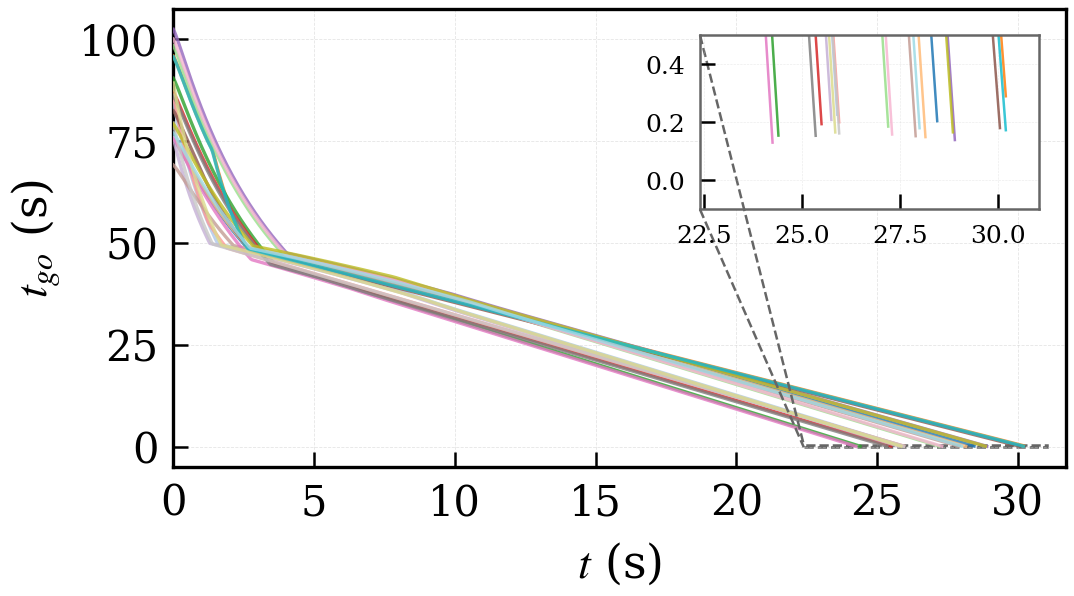
\includegraphics[width=3.2in]{mappo_nopn_tgo.png}
\caption{Time-to-go ($t_{go}$) profiles of the defending swarm using ART-MAPPO in Case~1. Interceptors assigned to the same target actively synchronize their remaining flight times to guarantee a simultaneous saturation strike.}
\label{fig:case1_mappo_tgo}
\end{figure}

Consequently, Fig.~\ref{fig:case1_time_sync} explicitly validates the ultimate temporal coordination capability by displaying the terminal arrival time difference ($\Delta t$) among the interceptors assigned to each respective target group. The maximum $\Delta t$ across all eight coordinated groups is remarkably tight, bounded to merely 0.45\,s. This quantitatively proves that the proposed framework perfectly bridges the target assignment and the trust-modulated exploration mechanisms, ensuring a strictly temporally coordinated saturation strike against the swarm threat.

\begin{figure}[!ht]
\centering
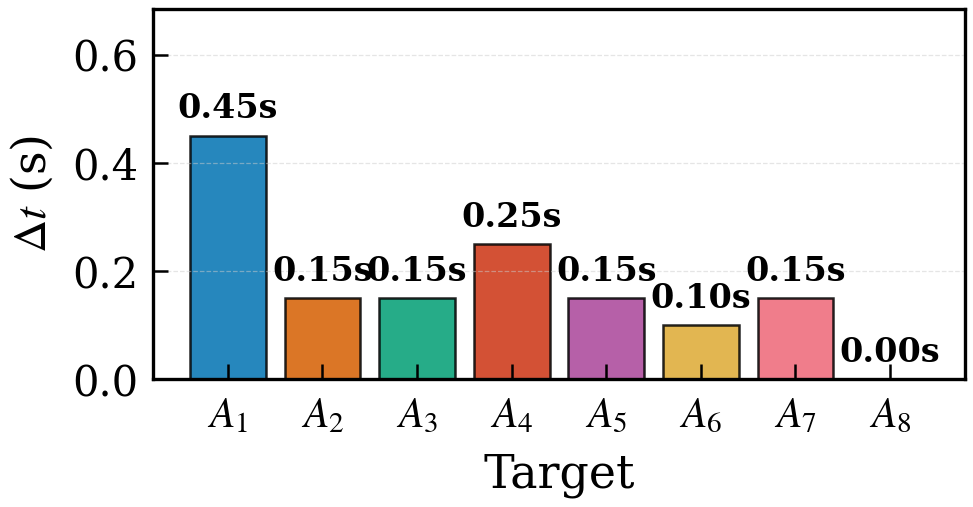
\includegraphics[width=3.0in]{mappo_success_nopn_time_sync.png}
\caption{Terminal arrival time differences $\Delta t$ within each coordinated interceptor group under ART-MAPPO. The near-zero $\Delta t$ values explicitly validate the successful execution of temporally synchronized saturation strikes.}
\label{fig:case1_time_sync}
\end{figure}







\subsubsection{Case~2: Interception against Continuous Weaving Targets}

This scenario evaluates the robustness of the proposed framework against the sinusoidal penetration maneuver~\cite{Zarchan1995969}, which represents a highly agile and continuous weaving threat. Such maneuvers induce high-frequency oscillations in the line-of-sight (LOS) rate, severely challenging both the guidance stability and the temporal coordination of the defending swarm.

The 2D engagement trajectories of the ART-MAPPO defending swarm are illustrated in Fig.~\ref{fig:case2_mappo_traj}. Despite the continuous lateral oscillations of the $A_{\text{UAV}}$, ART-MAPPO explicitly predicts and accommodates the target's weaving motion. The defending swarm maintains all eight coordinated combat units and successfully intercepts every target with smooth pursuit curves.

\begin{figure}[!ht]
\centering
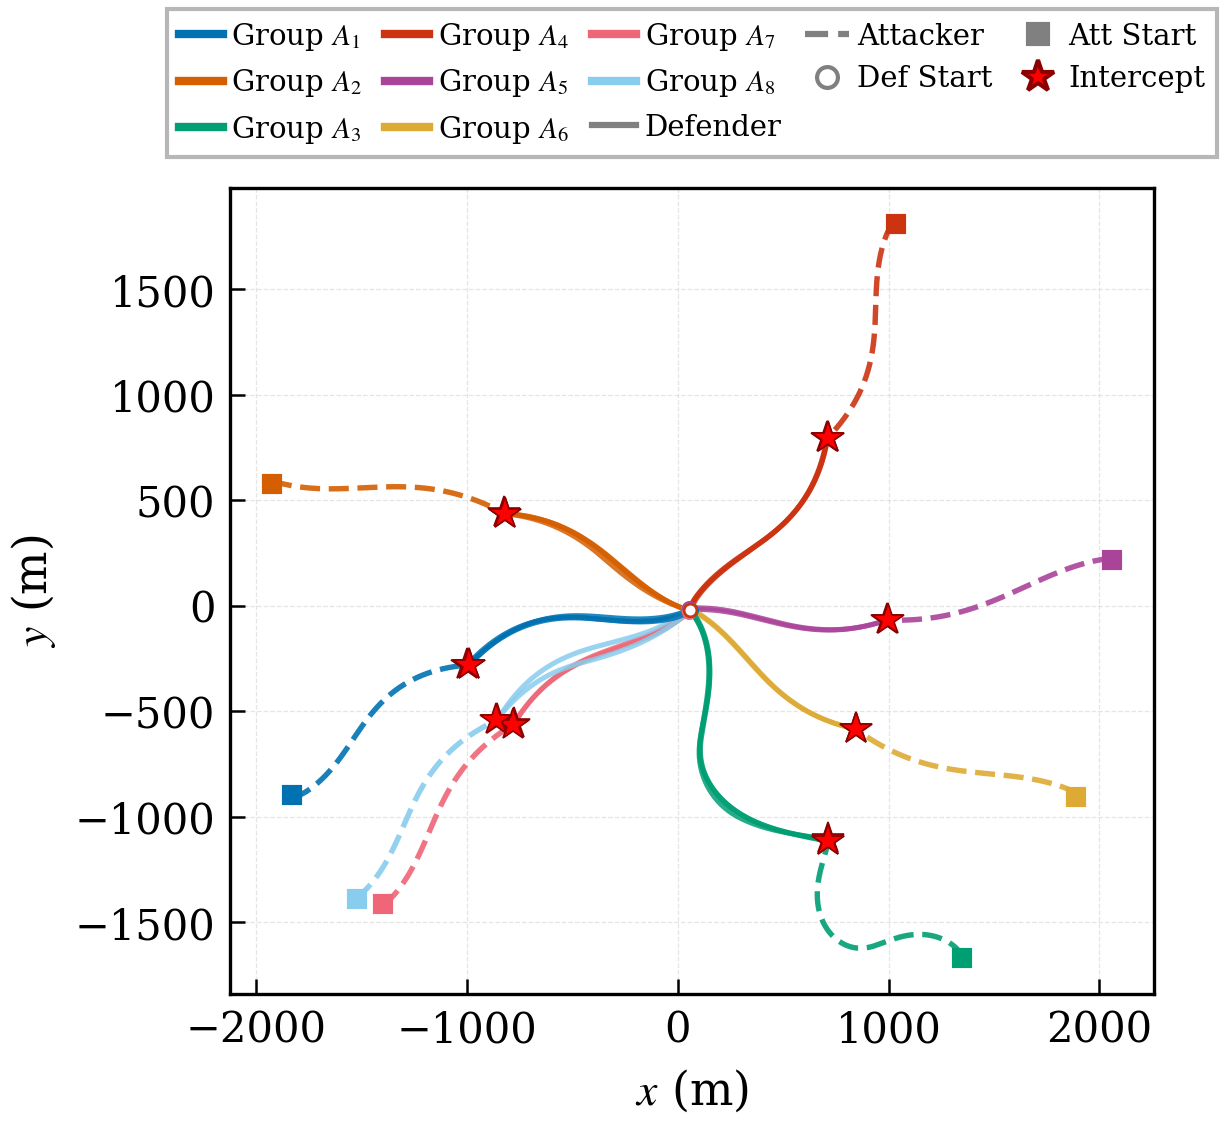
\includegraphics[width=3.2in]{mappo_sin_trajectory.png}
\caption{Engagement trajectories of the defending swarm using ART-MAPPO against continuous weaving targets (Case~2).}
\label{fig:case2_mappo_traj}
\end{figure}

The underlying kinematic and control mechanisms of ART-MAPPO are further detailed in Fig.~\ref{fig:case2_mappo_kine}. The most significant advantage is observed in the normal acceleration profile ($n_y$) shown in Fig.~\ref{fig:case2_mappo_kine}(a). To counter the weaving target, ART-MAPPO generates an intelligent, adaptive oscillatory $n_y$ command that perfectly tracks the target's maneuvering frequency. Most importantly, it achieves this dynamic tracking while strictly remaining within the safe aerodynamic envelope ($\pm 1$\,g), completely averting terminal saturation. Furthermore, it smoothly adjusts its heading angle (Fig.~\ref{fig:case2_mappo_kine}(b)). Similar to Case~1, ART-MAPPO aggressively leverages its axial acceleration ($n_x$) to maximize approach velocity, as demonstrated in the velocity and axial acceleration profiles (Fig.~\ref{fig:case2_mappo_kine}(c) and (d)).

\begin{figure}[!ht]
\centering

\includegraphics[width=3.0in]{standalone_duav_legend.png}
\subfloat[Normal acceleration $n_y$]{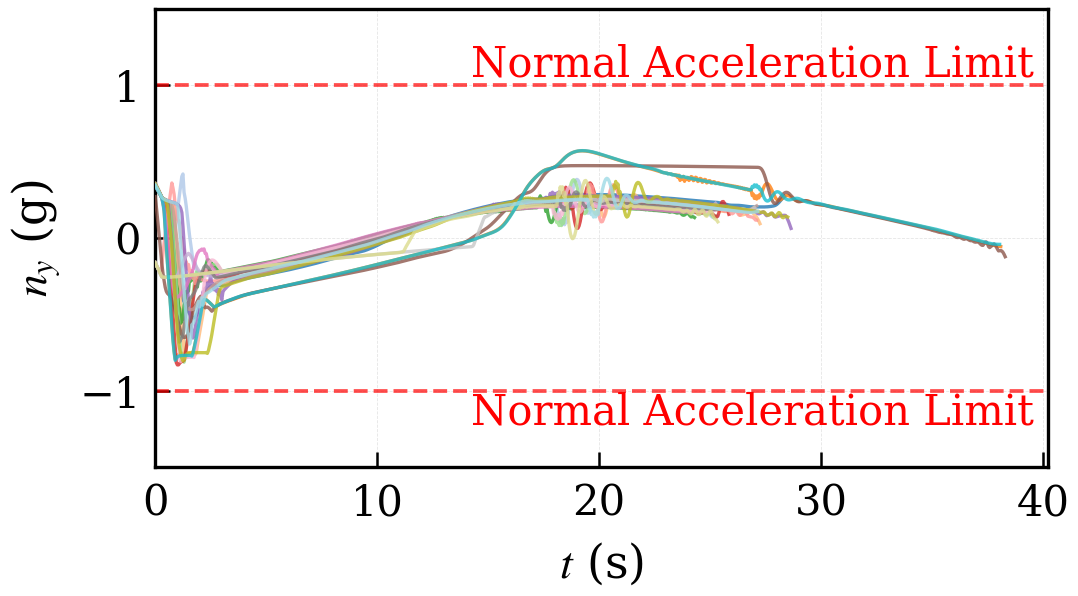
\includegraphics[width=3.0in]{mappo_sin_ny.png}}
\hfil
\subfloat[Heading angle $\gamma_D$]{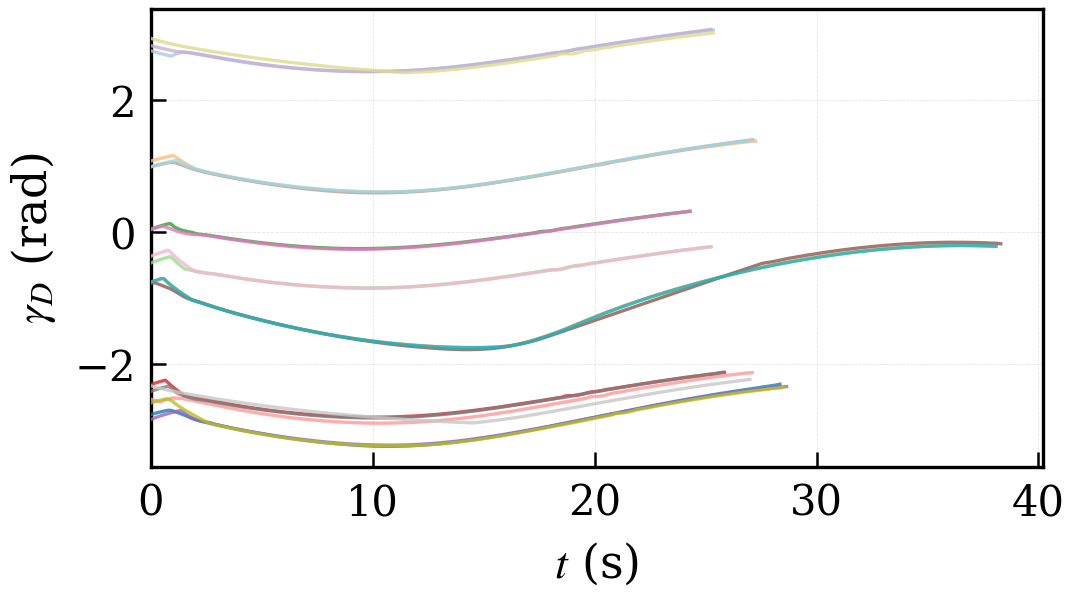
\includegraphics[width=3.0in]{mappo_sin_heading.png}}
\hfil
\subfloat[Velocity $V_D$]{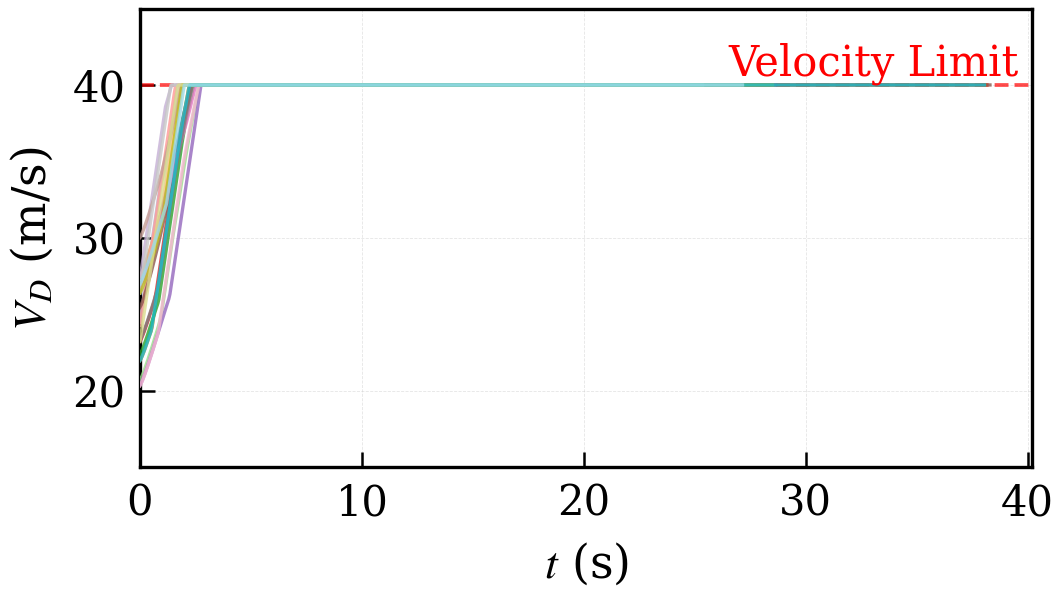
\includegraphics[width=3.0in]{mappo_sin_velocity.png}}
\hfil
\subfloat[Axial acceleration $n_x$]{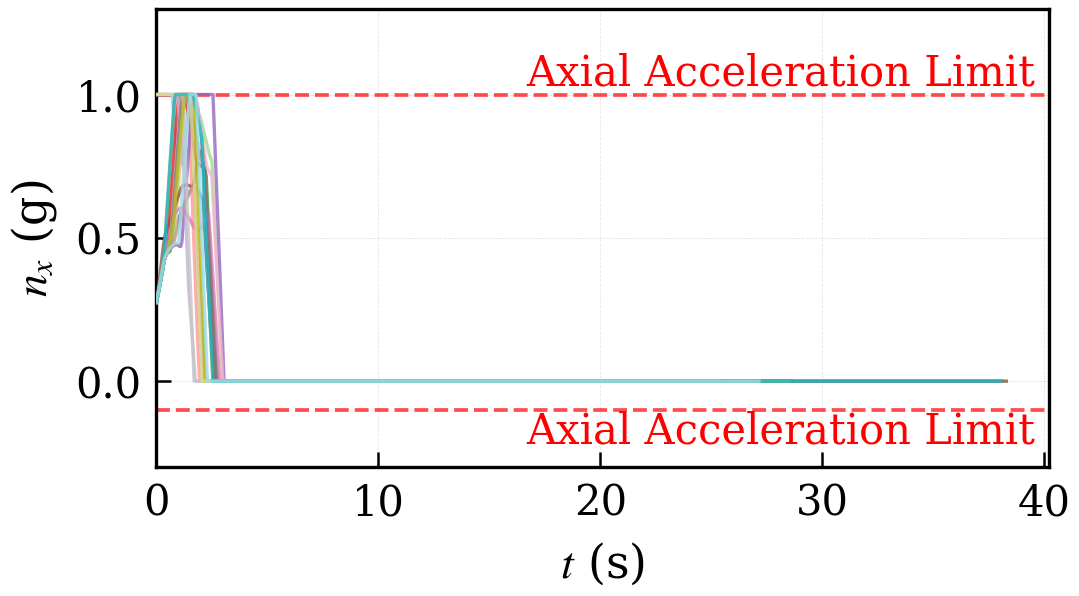
\includegraphics[width=3.0in]{mappo_sin_nx.png}}
\vspace{0pt}
\caption{Kinematic and control effort profiles of ART-MAPPO for Case~2. The policy dynamically outputs adaptive oscillatory normal commands ($n_y$) to track the weaving target without violating the $\pm1$\,g limit.}
\label{fig:case2_mappo_kine}
\end{figure}

Conversely, the PN baseline completely fails to handle the high-frequency dynamic engagement geometry. The reactive nature of PN results in phase-lagged trajectories that struggle to close the distance (Fig.~\ref{fig:case2_pn_traj}). As revealed in the control profiles (Fig.~\ref{fig:case2_pn_kine}), the PN guidance law suffers from catastrophic actuator saturation during the terminal phase. Specifically, the normal commands ($n_y$) frequently breach the $\pm 1$\,g limit (Fig.~\ref{fig:case2_pn_kine}(a)), which would severely compromise flight safety and render the interception a failure in real-world applications.

\begin{figure}[!ht]
\centering

\includegraphics[width=3.2in]{pn_sin_trajectory.png}
\caption{Engagement trajectories of the defending swarm using the PN baseline in Case~2.}
\label{fig:case2_pn_traj}
\end{figure}

\begin{figure}[!ht]
\centering

\includegraphics[width=3.0in]{standalone_duav_legend.png}
\subfloat[Normal acceleration $n_y$]{
\includegraphics[width=3.0in]{pn_sin_ny.png}}
\hfil
\subfloat[Heading angle $\gamma_D$]{
\includegraphics[width=3.0in]{pn_sin_heading.png}}
\hfil
\subfloat[Velocity $V_D$]{
\includegraphics[width=3.0in]{pn_sin_velocity.png}}
\hfil
\subfloat[Axial acceleration $n_x$]{
\includegraphics[width=3.0in]{pn_sin_nx.png}}
\vspace{0pt}
\caption{Kinematic and control effort profiles of the PN baseline for Case~2, highlighting catastrophic terminal actuator saturation ($n_y$ significantly exceeding limits).}
\label{fig:case2_pn_kine}
\end{figure}

The continuous maneuvering of the targets also disrupts conventional coordination mechanisms. However, this vital temporal synchronization is dynamically sustained by ART-MAPPO during the flight, as evidenced by the time-to-go ($t_{go}$) profiles in Fig.~\ref{fig:case2_mappo_tgo}. Even against severe LOS oscillations, the $t_{go}$ curves of interceptors assigned to the same target smoothly converge. This demonstrates that the algorithm continuously and intelligently adapts the swarm's velocity distribution to lock in synchronized impact times, despite the highly dynamic nature of the weaving threats.

\begin{figure}[!ht]
\centering
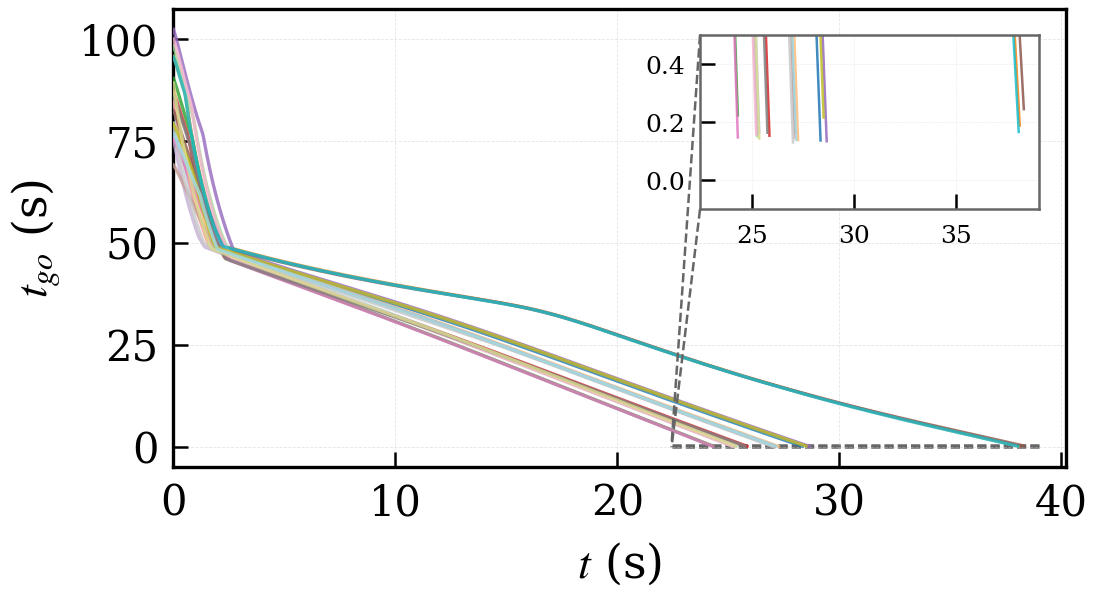
\includegraphics[width=3.2in]{mappo_sin_tgo.png}
\caption{Time-to-go ($t_{go}$) profiles of the defending swarm using ART-MAPPO in Case~2. Interceptors actively synchronize their remaining flight times despite the continuous high-G maneuvers of the targets.}
\label{fig:case2_mappo_tgo}
\end{figure}

Consequently, the ultimate validation of ART-MAPPO's saturation strike capability under extreme dynamic conditions is explicitly presented in Fig.~\ref{fig:case2_time_sync}. Even against highly evasive sinusoidal targets, the maximum terminal arrival time difference ($\Delta t$) among the coordinated groups is strictly bounded to 0.30\,s. This exceptional synchronization quantitatively confirms the superiority of the ART-MAPPO framework in executing temporally coordinated saturation strikes in highly complex adversarial environments.

\begin{figure}[!ht]
\centering
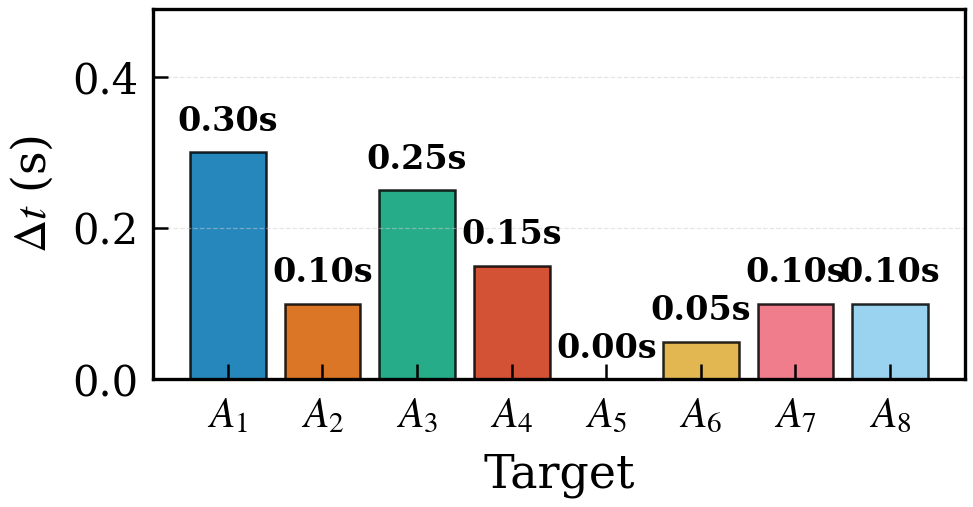
\includegraphics[width=3.0in]{mappo_success_sin_time_sync.png}
\caption{Terminal arrival time differences $\Delta t$ for Case~2. The remarkably low variance ($\le 0.30$\,s) proves that ART-MAPPO preserves strict temporal synchronization even against continuous weaving targets.}
\label{fig:case2_time_sync}
\end{figure}







\subsection{Monte Carlo Statistical Analysis and Robustness}
\label{subsec:montecarlo}

To rigorously quantify the robustness of the proposed framework, 1000 independent Monte Carlo trials are conducted for each case. It is important to note that the statistical distributions presented in Fig.~\ref{fig:mc_boxplots} ($E_{co\text{-}time}$, $E_n$, $E_{miss}$, and $E_t$) are exclusively derived from the successful interception trials. Specifically, out of the 1000 trials in Case~1, ART-MAPPO and PN successfully intercepted the targets 987 and 944 times, respectively. In the highly dynamic Case~2, ART-MAPPO maintained a remarkable 971 successful interceptions, whereas the baseline PN succeeded only 175 times. 

\begin{figure}[!t]
\centering
\subfloat[Case~1]{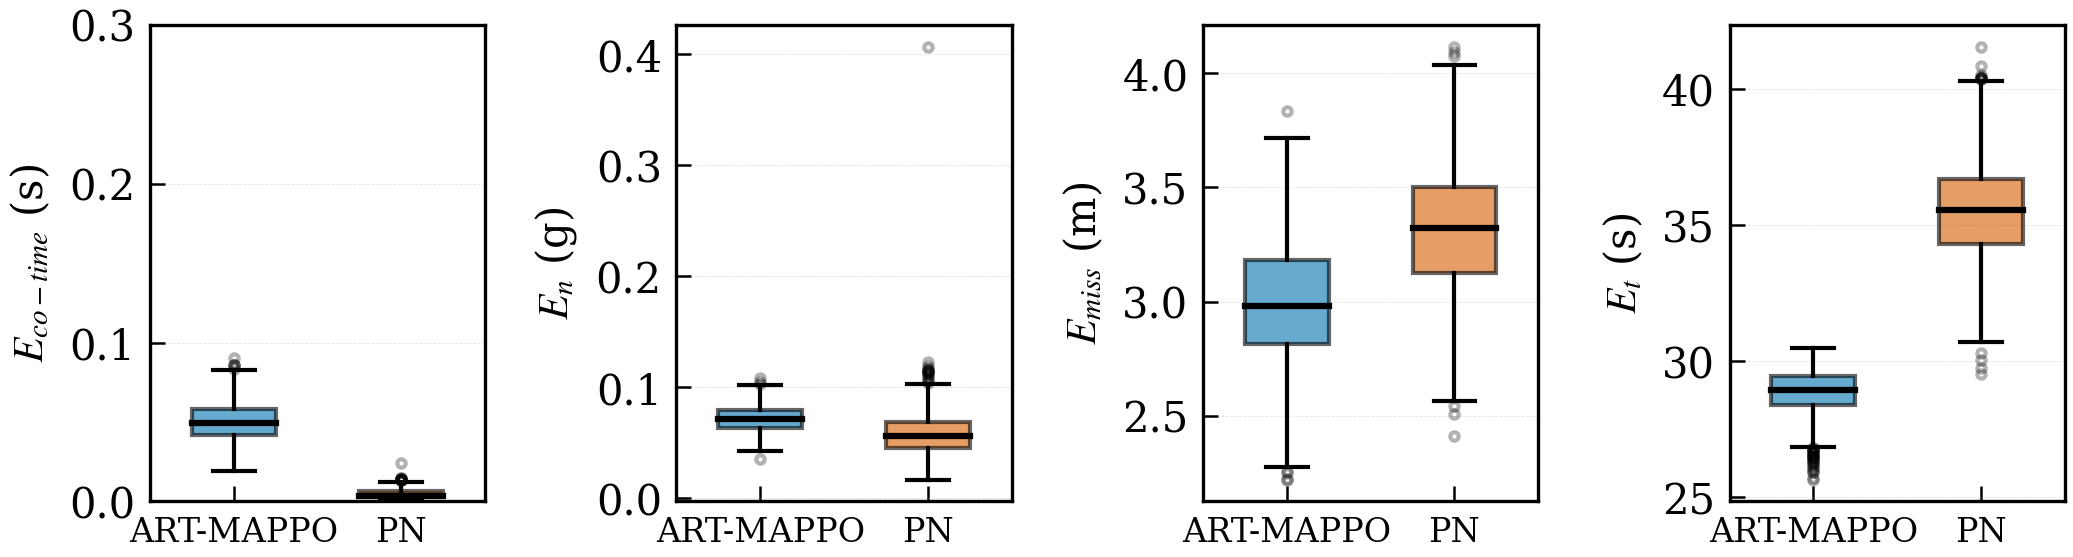
\includegraphics[width=3.5in]{nopn_mc_boxplot_compare.png}}\\
\subfloat[Case~2]{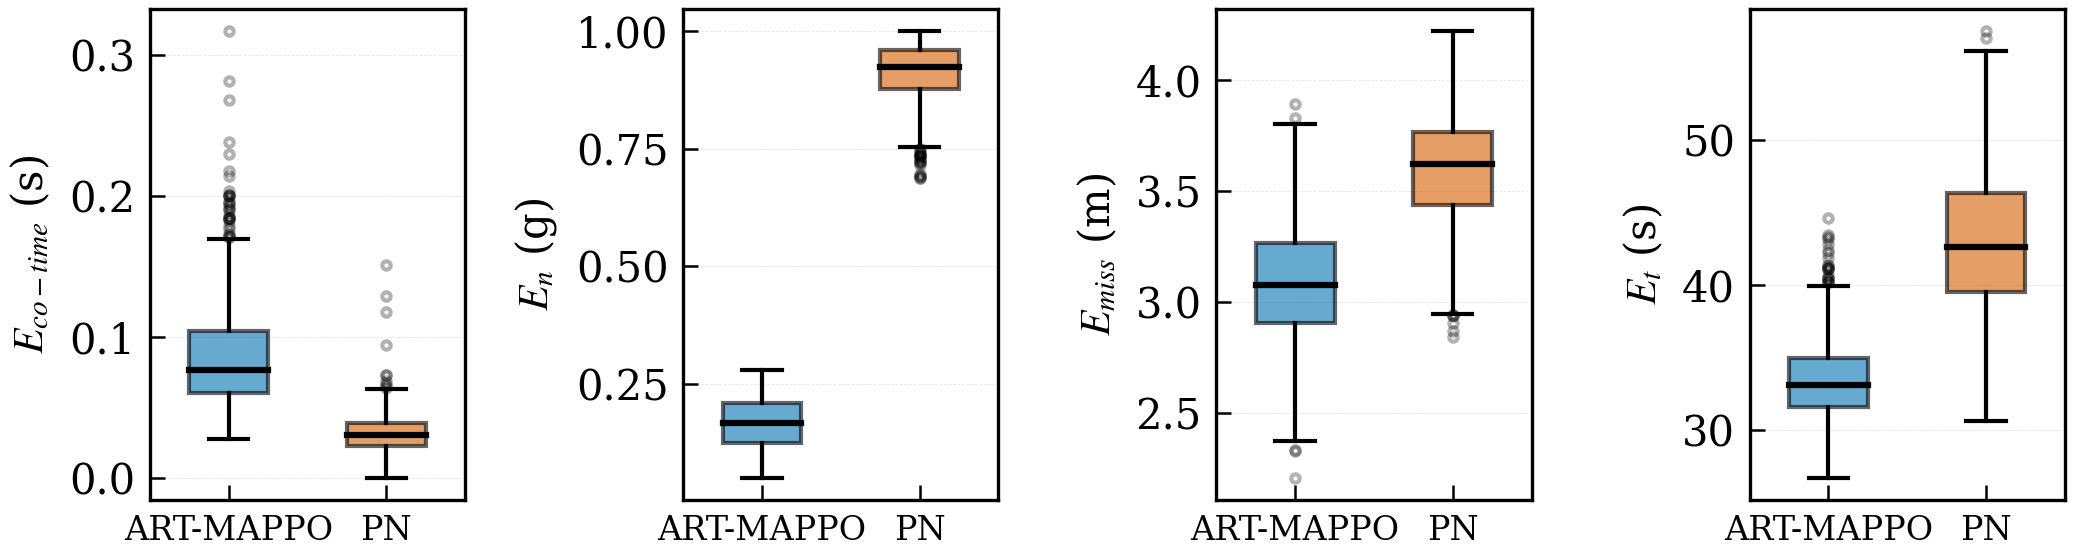
\includegraphics[width=3.5in]{sin_mc_boxplot_compare.png}}
\caption{Boxplots of Monte Carlo trials comparing ART-MAPPO and PN (data derived from successful interceptions).}
\label{fig:mc_boxplots}
\end{figure}

Based on the statistical distributions, three key findings emerge:

\emph{(i) Interception reliability and precision.} The Interception Success Rates (ISRs) directly reflect the algorithms' adaptability to aggressive target maneuvers. While PN achieves a respectable 94.40\% against the evasive target (Case~1), its performance precipitously degrades to 17.50\% when facing the continuous weaving target (Case~2). Conversely, ART-MAPPO sustains exceptional ISRs of 98.70\% and 97.14\%, demonstrating profound robustness against continuous, high-frequency line-of-sight (LOS) oscillations. Furthermore, the $E_{miss}$ boxplots confirm that ART-MAPPO consistently achieves a lower median miss distance with a significantly narrower interquartile range (IQR), ensuring lethal precision even under worst-case initializations.

\emph{(ii) Terminal required overload and operational efficiency.} The metric $E_n$ denotes the terminal required normal overload, which is a critical constraint for flight safety. As depicted in the boxplots, ART-MAPPO's $E_n$ is tightly clustered around a safe median of $\approx0.08$\,g (Case~1) and $\approx0.20$\,g (Case~2). In stark contrast, particularly in Case~2, PN's $E_n$ distribution is heavily squeezed near the 1.0\,g upper bound. This exposes severe terminal actuator saturation, as PN struggles to reactively track the sinusoidal maneuvers. Additionally, ART-MAPPO strictly bounds the engagement duration ($E_t$) within a tight and predictable time window, reflecting superior forward energy management and rapid closure capabilities.

\emph{(iii) Robust temporal coordination.} The metric $E_{co\text{-}time}$ evaluates the temporal synchronization of the defending swarm. Across the successful Monte Carlo trials in both highly dynamic scenarios, ART-MAPPO maintains a median $E_{co\text{-}time}$ well below 0.10\,s. This consistently tight distribution confirms that the proposed algorithm can reliably shape the swarm's velocity profile to satisfy the strict temporal requirements for simultaneous saturation strikes, effectively neutralizing the risk of sequential piecemeal defeat.



%% ===========================================================
\section{Conclusion}
\label{sec:conclusion}

In this paper, the cooperative interception problem of UAV swarms against highly dynamic and
maneuverable attacking UAV swarms has been investigated, explicitly accounting for real-time
decision requirements, coordinated engagement effectiveness, and terminal overload risk.
The problem is formulated by jointly considering target assignment and cooperative guidance,
and an intelligent temporally coordinated interception framework is developed.
A fast IDBO-based target assignment mechanism enables efficient and accurate resource
allocation in dynamic environments.
The ART-MAPPO cooperative guidance strategy under the CTDE paradigm improves learning
stability and training efficiency in large-scale adversarial settings.
Extensive simulations demonstrate accelerated target assignment, enhanced interception
efficiency, improved interception success rates, and effective alleviation of terminal overload
saturation.

For future work, promising directions include cooperative interception under incomplete
information, dynamic target reassignment in unknown environments, time-constrained assignment
with explicit completion deadlines, and integration with realistic constraints such as
communication delays, limited bandwidth, and heterogeneous UAV capabilities.

% ---- Bibliography ----
\bibliographystyle{IEEEtran}
\bibliography{cja-template}

\end{document}
